%%**************************************************************
%% Vorlage fuer Bachelorarbeiten (o.ä.) der DHBW
%%
%% Autor: Tobias Dreher, Yves Fischer
%% Datum: 06.07.2011
%%
%% Autor: Michael Gruben
%% Datum: 15.05.2013
%%
%% Autor: Markus Barthel
%% Datum: 22.08.2014
%%**************************************************************

\input{ads/header}

\makeglossaries
%!TEX root = ../dokumentation.tex

%
% vorher in Konsole folgendes aufrufen:
%	makeglossaries makeglossaries dokumentation.acn && makeglossaries dokumentation.glo
%

%
% Glossareintraege --> referenz, name, beschreibung
% Aufruf mit \gls{...}
%
\newglossaryentry{Glossareintrag}{name={Glossareintrag},plural={Glossareinträge},description={Ein Glossar beschreibt verschiedenste Dinge in kurzen Worten}}
\newglossaryentry{IntelliJ}{name={IntelliJ},description={Eine Programmierumgebung für Java Projekte}}
\newglossaryentry{Springboot}{name={Springboot},description={\glqq{Spring Boot makes it easy to create stand-alone, production-grade Spring based Applications that you can \lq{just run}\rq{}.}\grqq{}}\cite[]{Springboot}}
\newglossaryentry{Terraform}{name={Terraform},description={folgt\dots}}
\newglossaryentry{Spring}{name={Spring},description={\glqq{The Spring Framework provides a comprehensive programming and configuration model for modern Java-based enterprise applications - on any kind of deployment platform.}\grqq{}}\cite[]{Spring}}
\newglossaryentry{Box}{name={Box},description={folgt\dots}}

\begin{document}

	% Deckblatt
	\begin{spacing}{1}
		%!TEX root = ../dokumentation.tex

\begin{titlepage}
	\begin{longtable}{p{8.2cm} p{5.4cm}}
		{\raisebox{\ht\strutbox-\totalheight}{
\includegraphics[height=2.5cm]{images/firma-deckblatt.png}}} &
		{\raisebox{\ht\strutbox-\totalheight}{\includegraphics[height=2.5cm]{images/dhbw.png}}}
	\end{longtable}
	\enlargethispage{20mm}
	\begin{center}
		\vspace*{12mm}	{\LARGE\textbf \titel }\\
		\vspace*{12mm}	{\large\textbf \arbeit}\\
		\vspace*{12mm}	\langdeckblattabschlusshinleitung\\
		\vspace*{3mm}		{\textbf \abschluss}\\
		\vspace*{12mm}	\langartikelstudiengang{} \langstudiengang{} \studiengang\\
    \vspace*{3mm}		\langanderdh{} \dhbw\\
		\vspace*{12mm}	\langvon\\
		\vspace*{3mm}		{\large\textbf \autor}\\
		\vspace*{12mm}	\datumAbgabe\\
	\end{center}
	\vfill
	\begin{spacing}{1.2}
	\begin{tabbing}
		mmmmmmmmmmmmmmmmmmmmmmmmmm             \= \kill
		\textbf{\langdbbearbeitungszeit}       \>  \zeitraum\\
		\textbf{\langdbmatriknr, \langdbkurs}  \>  \matrikelnr, \kurs\\
		\textbf{\langdbfirma}                  \>  \firma, \firmenort\\
		\textbf{\langdbbetreuer}               \>  \betreuer\\
		\textbf{\langdbgutachter}              \>  \gutachter
	\end{tabbing}
	\end{spacing}
\end{titlepage}

	\end{spacing}
	\newpage

	\pagenumbering{Roman}

	% Sperrvermerk
	% \input{ads/sperrvermerk}
	\newpage

	% Erklärung
	%!TEX root = ../dokumentation.tex

\thispagestyle{empty}

\section*{\langerklaerung}
\vspace*{2em}

\iflang{de}{%
Ich versichere hiermit, dass ich meine {\arbeit} mit dem Thema: {\itshape \titel } selbstständig verfasst und keine anderen als die angegebenen Quellen und Hilfsmittel benutzt habe.
% Ich versichere zudem, dass die eingereichte elektronische Fassung mit der gedruckten Fassung übereinstimmt. 

% https://www.dhbw-karlsruhe.de/fileadmin/user_upload/dokumente/T-Informatik/Prüfungsordnung-Technik-2015-09-29.pdf (S. 19)
% https://www.dhbw-stuttgart.de/fileadmin/dateien/Amtliche_Bekanntmachungen/20_2017_Bekanntmachung_StuPrO_DHBW_Technik.pdf (S. 21)


% Ich erkläre hiermit ehrenwörtlich: \\
% \begin{enumerate}
% \item dass ich meine {\arbeit} mit dem Thema
% {\itshape \titel } ohne fremde Hilfe angefertigt habe;
% \item dass ich die Übernahme wörtlicher Zitate aus der Literatur sowie die Verwendung der Gedanken
% anderer Autoren an den entsprechenden Stellen innerhalb der Arbeit gekennzeichnet habe;
% \item dass ich meine {\arbeit} bei keiner anderen Prüfung vorgelegt habe;
% \item dass die eingereichte elektronische Fassung exakt mit der eingereichten schriftlichen Fassung
% übereinstimmt.
% \end{enumerate}
% 
% Ich bin mir bewusst, dass eine falsche Erklärung rechtliche Folgen haben wird.

% % http://www.ib.dhbw-mannheim.de/fileadmin/ms/bwl-ib/Downloads_alt/Leitfaden_31.05.pdf (S. 52)
}


\iflang{en}{%
Hereby I solemnly declare:
\begin{enumerate}
\item that this {\arbeit}, titled {\itshape \titel } is entirely the product of my own scholarly work, unless otherwise indicated in the text or references, or acknowledged below;
\item I have indicated the thoughts adopted directly or indirectly from other sources at the appropriate places within the document;
\item this {\arbeit} has not been submitted either in whole or part, for a degree at this or any other university or institution;
\item I have not published this {\arbeit} in the past; 
\item the printed version is equivalent to the submitted electronic one.
\end{enumerate}
I am aware that a dishonest declaration will entail legal consequences.
}

\vspace{3em}

\abgabeort, \datumAbgabe
\vspace{4em}
\begin{figure}[H]

\includegraphics[width=0.3\textwidth]{signature.png}
\end{figure}
\rule{6cm}{0.4pt}\\
\autor

	\newpage

	% Gender-Disclaimer
	% !TeX root = ../dokumentation.tex

\thispagestyle{empty}

\section*{Gender-Disclaimer}

In dieser Arbeit wird aus Gründen der besseren Lesbarkeit das generische Maskulinum
verwendet. Weibliche und anderweitige Geschlechteridentitäten werden dabei
ausdrücklich mitgemeint, soweit es für die Aussage erforderlich ist.
	\newpage

	% Abstract
	%!TEX root = ../dokumentation.tex

\pagestyle{empty}

\iflang{de}{%
% Dieser deutsche Teil wird nur angezeigt, wenn die Sprache auf Deutsch eingestellt ist.
\renewcommand{\abstractname}{\langabstract} % Text für Überschrift

% \begin{otherlanguage}{english} % auskommentieren, wenn Abstract auf Deutsch sein soll
\begin{abstract}
Um eine lokale anwendung unternehmensintern weltweit ohne Installation verfügbar zu machen,
ist eine Transformation dieser in die Cloud ein mögliches Konzept, um dies umzusetzen.
Eine solche Transformation bringt sowohl Vor- als auch Nachteile mit sich, die in der Arbeit untersucht werden sollen.
Dazu wird eine Use Case Analyse anhand der Durchführung einer Transformation für eine Financial Management Anwendung,
ein Vergleich der Services möglicher verschiedener Cloudanbieter und eine empirische Analyse in Form von Auswertung von
Statistiken zu aktuellen Trends und möglicher Effizienzsteigerung in der Cloud Transformation durchgeführt.
Ziel ist es, die Vor- und Nachteile aus der Analyse herauszuarbeiten und einen kleinen Einblick in die tatsächliche
Dürchführung der Anwendungstransformation zu geben.

\end{abstract}
% \end{otherlanguage} % auskommentieren, wenn Abstract auf Deutsch sein soll
}



\iflang{en}{%
% Dieser englische Teil wird nur angezeigt, wenn die Sprache auf Englisch eingestellt ist.
\renewcommand{\abstractname}{\langabstract} % Text für Überschrift

\begin{abstract}
An abstract is a brief summary of a research article, thesis, review, conference proceeding or any in-depth analysis of a particular subject or discipline, and is often used to help the reader quickly ascertain the paper's purpose. When used, an abstract always appears at the beginning of a manuscript, acting as the point-of-entry for any given scientific paper or patent application. Abstracting and indexing services for various academic disciplines are aimed at compiling a body of literature for that particular subject.

The terms précis or synopsis are used in some publications to refer to the same thing that other publications might call an ``abstract''. In ``management'' reports, an executive summary usually contains more information (and often more sensitive information) than the abstract does.

Quelle: \url{http://en.wikipedia.org/wiki/Abstract_(summary)}

\end{abstract}
}
	\newpage

	\pagestyle{plain}		% nur Seitenzahlen im Fuß
	
	\RedeclareSectionCommand[beforeskip=\kapitelabstand         ]{chapter} % stellt Abstand vor Kapitelüberschriften ein

	% Inhaltsverzeichnis
	\begin{spacing}{1.1}
		\begingroup
		
			% auskommentieren für Seitenzahlen unter Inhaltsverzeichnis
			\renewcommand*{\chapterpagestyle}{empty}
			\pagestyle{empty}
			
			
			\setcounter{tocdepth}{1}
			%für die Anzeige von Unterkapiteln im Inhaltsverzeichnis
			%\setcounter{tocdepth}{2}
			
			\tableofcontents
			\clearpage
		\endgroup
	\end{spacing}
	\newpage

	% Abkürzungsverzeichnis
	\cleardoublepage
	\thispagestyle{plain}
	\addchap{\langabkverz}
%nur verwendete Akronyme werden letztlich im Abkürzungsverzeichnis des Dokuments angezeigt
%Verwendung: 
%		\ac{Abk.}   --> fügt die Abkürzung ein, beim ersten Aufruf wird zusätzlich automatisch die ausgeschriebene Version davor eingefügt bzw. in einer Fußnote (hierfür muss in header.tex \usepackage[printonlyused,footnote]{acronym} stehen) dargestellt
%		\acs{Abk.}   -->  fügt die Abkürzung ein
%		\acf{Abk.}   --> fügt die Abkürzung UND die Erklärung ein
%		\acl{Abk.}   --> fügt nur die Erklärung ein
%		\acp{Abk.}  --> gibt Plural aus (angefügtes 's'); das zusätzliche 'p' funktioniert auch bei obigen Befehlen
%	siehe auch: http://golatex.de/wiki/%5Cacronym
%	
\begin{acronym}[YTMMM]
\setlength{\itemsep}{-\parsep}

\acro{AGPL}{Affero GNU General Public License}
\acro{WSN}{Wireless Sensor Network}
\acro{MANET}{Mobile wireless Ad-hoc NETwork}
\acro{MAC}{Multiple Access Control}
\acro{QoS}{Quality of Service}
\acro{DSR}{Dynamic Source Routing}
\acro{API}{Application Programming Interface}
\acro{WYSIWYG}{What You See Is What You Get}
\acro{HTML}{HyperText Markup Language}
\acro{SaaS}{Software-as-a-Service}
\acro{PaaS}{Platform-as-a-Service}
\acro{IaaS}{Infrastructure-as-a-Service}
\acro{CaaS}{Container-as-a-Service}
\acro{BaaS}{Backend-as-a-Service}
\acro{FaaS}{Functions-as-a-Service}
\acro{XaaS}{Everything-as-a-Service}
\acro{AWS}{Amazon Web Services}
\acro{NIST}{National Institute of Standards and Technology}
\acro{VPN}{Virtual Private Network}
\acro{REST}{Representational State Transfer}
\acro{JSON}{JavaScript Object Notation}
\acro{ECS}{Elastic Container Services}
\acro{VPC}{Virtual Private Cloud}
\acro{ECR}{Elastic Container Registry}
\acro{CI/CD}{Continuous Integration / Continuous Deployment}

\end{acronym}


	% Abbildungsverzeichnis
	\cleardoublepage
	\listoffigures

	%Tabellenverzeichnis
	\cleardoublepage
	\listoftables

	% Quellcodeverzeichnis
	\cleardoublepage
	\lstlistoflistings
	\cleardoublepage

	\pagenumbering{arabic}
	
	\pagestyle{headings}		% Kolumnentitel im Kopf, Seitenzahlen im Fuß

	% Inhalt
	% \foreach \i in {01,02,03,04,05,06,07,08,09,...,99} {%
	% 	\edef\FileName{content/\i kapitel}%
	% 		\IfFileExists{\FileName}{%
	% 			\input{\FileName}
	% 		}
	% 		{%
	% 			%file does not exist
	% 		}
	% }

	%!TEX root = ../../dokumentation.tex

\chapter{Einleitung}
% Erste Erwähnung eines Akronyms wird als Fußnote angezeigt. Jede weitere wird
% nur verlinkt: \acf{AGPL}. % \cite{fsf:2007}

% Verweise auf das Glossar: \gls{Glossareintrag}, \glspl{Glossareintrag}

Motivation:
Steigende Nutzerzahlen und zunehmende Digitalisierung bringen nach Hentschel und Leyh (2018) einen wachsenden Bedarf an
Rechenleistung und immer höhere Anforderungen an Informationssysteme mit sich, denen klassische Modelle der Datenverarbeitung
nicht mehr gerecht werden können. Cloud Computing dagegen ist durch Charakteristika wie Ressourcen Pooling und Elastizität \cite[Vgl.][S. 2]{Mell2011} in der Lage diese Anforderungen zu erfüllen
\cite[Vgl.][S. 6]{Reinheimer2018}.

Problemstellung:
Der zuor gezeigte, anhaltende Trend Anwendungen in der Cloud laufen zu lassen führt auch dazu,
dass legacy Anwendungen nach und nach in die Cloud Migriert werden.
Nach Kazanavičius, et al. (2019) stellt die Wahl der zum Unternehmen passenden Migrationsmethode
eine schwierige Aufgabe dar. Die erste Frage die hier beantwortet werden sollte sei demnach
"refactor or rebuild?" \cite[Vgl.][S. 4]{Kazanavicius2019}.
Darüber hinaus kommen auch Herausforderungen wie die Frage nach einem adäquaten Architekturdesign
für die Cloud \cite[Vgl.][S. 14]{Pahl} und der Untersuchng potenzieler Vor- und Nachteile
von zum Beispiel einer Microservice-Architektur und der Untersuchung möglicher Alternativen
\cite[Vgl.][S. 3]{Carrasco2018}.

Zielsetzung:
Aus der zuvor erarbeiteten Problemstellung ergibt sich als Ziel dieser Arbeit für
eine Unternehmensinterne, lokale Anwendung herauszuarbeiten, wie die Migration diese in die
Cloud vollzogen werden kann, welche Veränderungen in der Architektur und in Bezug auf die Benutzung
vorgenommen werden müssen und in welchen Aufgaben sich Herausforderungen befinden.

Out-of-Scope:
Explizit nicht betrachtet werden in dieser Arbeit die folgenden Aspekte:
\begin{itemize}
\item erstens
\item zweitens
\item drittens
\end{itemize}

\pagebreak

\section{Geschäftlicher Kontext}

In dieser Arbeit wird die Migration einer lokal laufenden Anwendung aus dem Projektmanagement zur Rechnungsstellung in die Cloud untersucht.
Zweck der Anwendung ist das Einsammeln sogenannter Timesheets von Projektmitarbeitern aus einem Cloud Speicher. Diese Timesheets dokumentieren,
wie viel Arbeitszeit ein Mitarbeiter für die verschiedenen Aufgaben in einem Projekt verbracht hat um daraus präzise Rechnungen erstellen zu können.

Das Tool wird bereits heute von mehreren Personen im Projekt verwendet und soll in Zukunft auch für andere Projekte eingesetzt werden. Aus diesem
Grund wird die Migration dieser Anwendung in die Cloud untersucht.

Die durchgeführte Migration soll die Anwendung daher global verfügbar machen und vorallem den Aufwand aber auch gegebenenfalls Kosten reduzieren.
Diese Anwendung muss bisher vom Anwender aus GitHub heruntergeladen und lokal ausgeführt werden.
Zur lokalen Ausführung sind einige Anpassungen in Konfigurationsdateien notwendig, da sich das ausführende System ändern kann.
Darüber hinaus muss die Anwendung nach jeder Aktualisierung manuell erneut heruntergeladen werden.
Das zur Verfügung stellen in der Cloud soll die Benutzung der Anwendung erleichtern und es auf lange Sicht ermöglichen, dass diese auch außerhalb der Projektumgebung verwendet werden kann.
\section{Einordnung dieser Arbeit in den wissenschaftlichen Kontext}

Grundlage für diese Arbeit bilden die zu dem Thema Cloud Migration veröffentlichten Publikationen, welche die Herausforderungen der Cloud Migration in Anbetracht der Wahl einer passenden Architektur erarbeiten. Dazu zählen unter anderem auch die Publikationen von Pahl et al., Carrasco et al. (2018) und Kazanavičius et al. (2019), die auf die Migration von \textit{legacy} Anwendungen in die Cloud eingehen und damit verbundene Herausforderungen aufzeigen. Dort wird unter anderem die Auswahl einer passenden Architektur \cite[Vgl.][S. 14]{Pahl}, der für das Unternehmen zutreffenden Migrationsstrategie \cite[Vgl.][S. 4]{Kazanavicius2019} und die Analyse potenzieller Vor- und Nachteile, von zum Beispiel der Microservice-Architektur \cite[Vgl.][S. 3]{Carrasco2018}, als Herausforderung erarbeitet.
\section{Kritische Auswahl der Forschungsmethoden}
\label{sec:auswahl_forschungsmethoden}

% Zielsetzung
% Literaturrecherche
% -hierzu zunächst aktuellen Stand der Forschung untersuchen
%  ->Thema x,y,z
% -Methodik beschreiben
% Anforderungsanalyse
% -non-functional Requirements
% -was muss beachtet werden für Cloud Anwendung
% -Anforderungen Cloud
% Use-Case Analyse
% -Werden Use-Cases immer noch erfüllt?
%  ->zufriedenstellend?
% -Architekturelle Änderungen (Client -> Web)
% Prototyping
% Evaluation

Um das Ziel dieser Arbeit zu erreichen wird zunächst der aktuelle Stand der wissenschaftlichen Forschung untersucht. Besonderer Fokus wird hierbei auf die Untersuchung der Herausforderungen der Cloud Migration, bevor die Durchführung eines Migrationsansatzes betrachtet wird.

Um die aktuellen Herausforderungen herauszuarbeiten wird eine Literaturrecherche nach Döring/Bortz 2016 durchgeführt. Dazu werden einige Suchbegriffe zur systematischen Durchsuchung wissenschaftlicher Datenbanken festgelegt \cite[Vgl.][S. 158]{Doering2016}. Als Suchmaschine wurde in diesem Fall hauptsächlich Google Scholar genutzt, da hierüber auch auf weitere Datenbanken verwiesen wird. Darüber hinaus wurde vor allem noch die Datenbank des Verlages Springer verwendet, aber vereinzelt auch noch einige weitere wie arXiv oder ACM.

Zur Recherche wurden die folgenden Begriffe verwendet: \glqq{Cloud Migration}\grqq{}, \glqq{Cloud Computing}\grqq{}, \glqq{Cloud}\grqq{}, \glqq{Herausforderungen Cloud Migration}\grqq{}

Diese werden als \textbf{\glqq{primäre Suchbegriffe}\grqq{}} \cite[S. 158]{Doering2016} festgelegt. Die Suche wurde darüber hinaus nach dem Schneeballsystem durchgeführt, was bedeutet, dass die Quellen der verwendeten Veröffentlichungen zur weiteren Recherche verwendet werden \cite[Vgl.][S. 160]{Doering2016}. Aus den Quellen werden außerdem weitere Begriffe als \textbf{\glqq{sekundäre Suchbegriffe}\grqq{}} \cite[S. 158]{Doering2016} festgelegt und zur erweiterten Suche verwendet. Zu diesen gehören unter anderem \glqq{Migration zu PaaS}\grqq, \glqq{Cloud Native}\grqq{} und \glqq{Refactoring}\grqq{}.

Außerdem wird das \textit{Prototyping} wie in Wilde/Hess 2007 und Heinrich 2011 beschrieben, zur Umsetzung des Anwendungsbeispiels und eine Use-Case Modellierung und Analyse dieser in Anbetracht der entwickelten Anwendung durchgeführt.
	%!TEX root = ../../dokumentation.tex

\chapter{Theoretische Grundlagen}
\label{chap:grundlagen}

Das folgende Kapitel bietet einen Überblick über den aktuellen Stand der Forschung und aktuelle Entwicklungen im Themenbereich des Cloud Computing und im Speziellen der Cloud Migration.

\section{Cloud Computing}

Im folgenden Unterkapitel werden die Grundlagen und eine Definition des Cloud Computing erarbeitet. Hierbei werden die Grundlegenden Konzepte, Bereitstellungsmodelle und Abstraktionsebenen des Cloud Computing erläutert.

\subsection{Was ist Cloud Computing}

Nach dem \ac{NIST}, auf dessen Definition sich in jüngerer Literatur häufig bezogen wird \cite[Vgl.][S. 4f]{Reinheimer2018}, ist Cloud Computing ein Modell der Zurverfügungstellung von Computing Ressourcen (z.B. Netzwerke, Server, Speicher, Anwendungen und Services),die über das Netzwerk erreichbar sind und mit geringem Managementaufwand schnell freigegeben und bereitgestellt werden können \cite[Vgl.][S. 2]{Mell2011}\cite[Vgl.][S. 5]{Reinheimer2018}.

\begin{wrapfigure}{r}{0.45\textwidth}
\centering
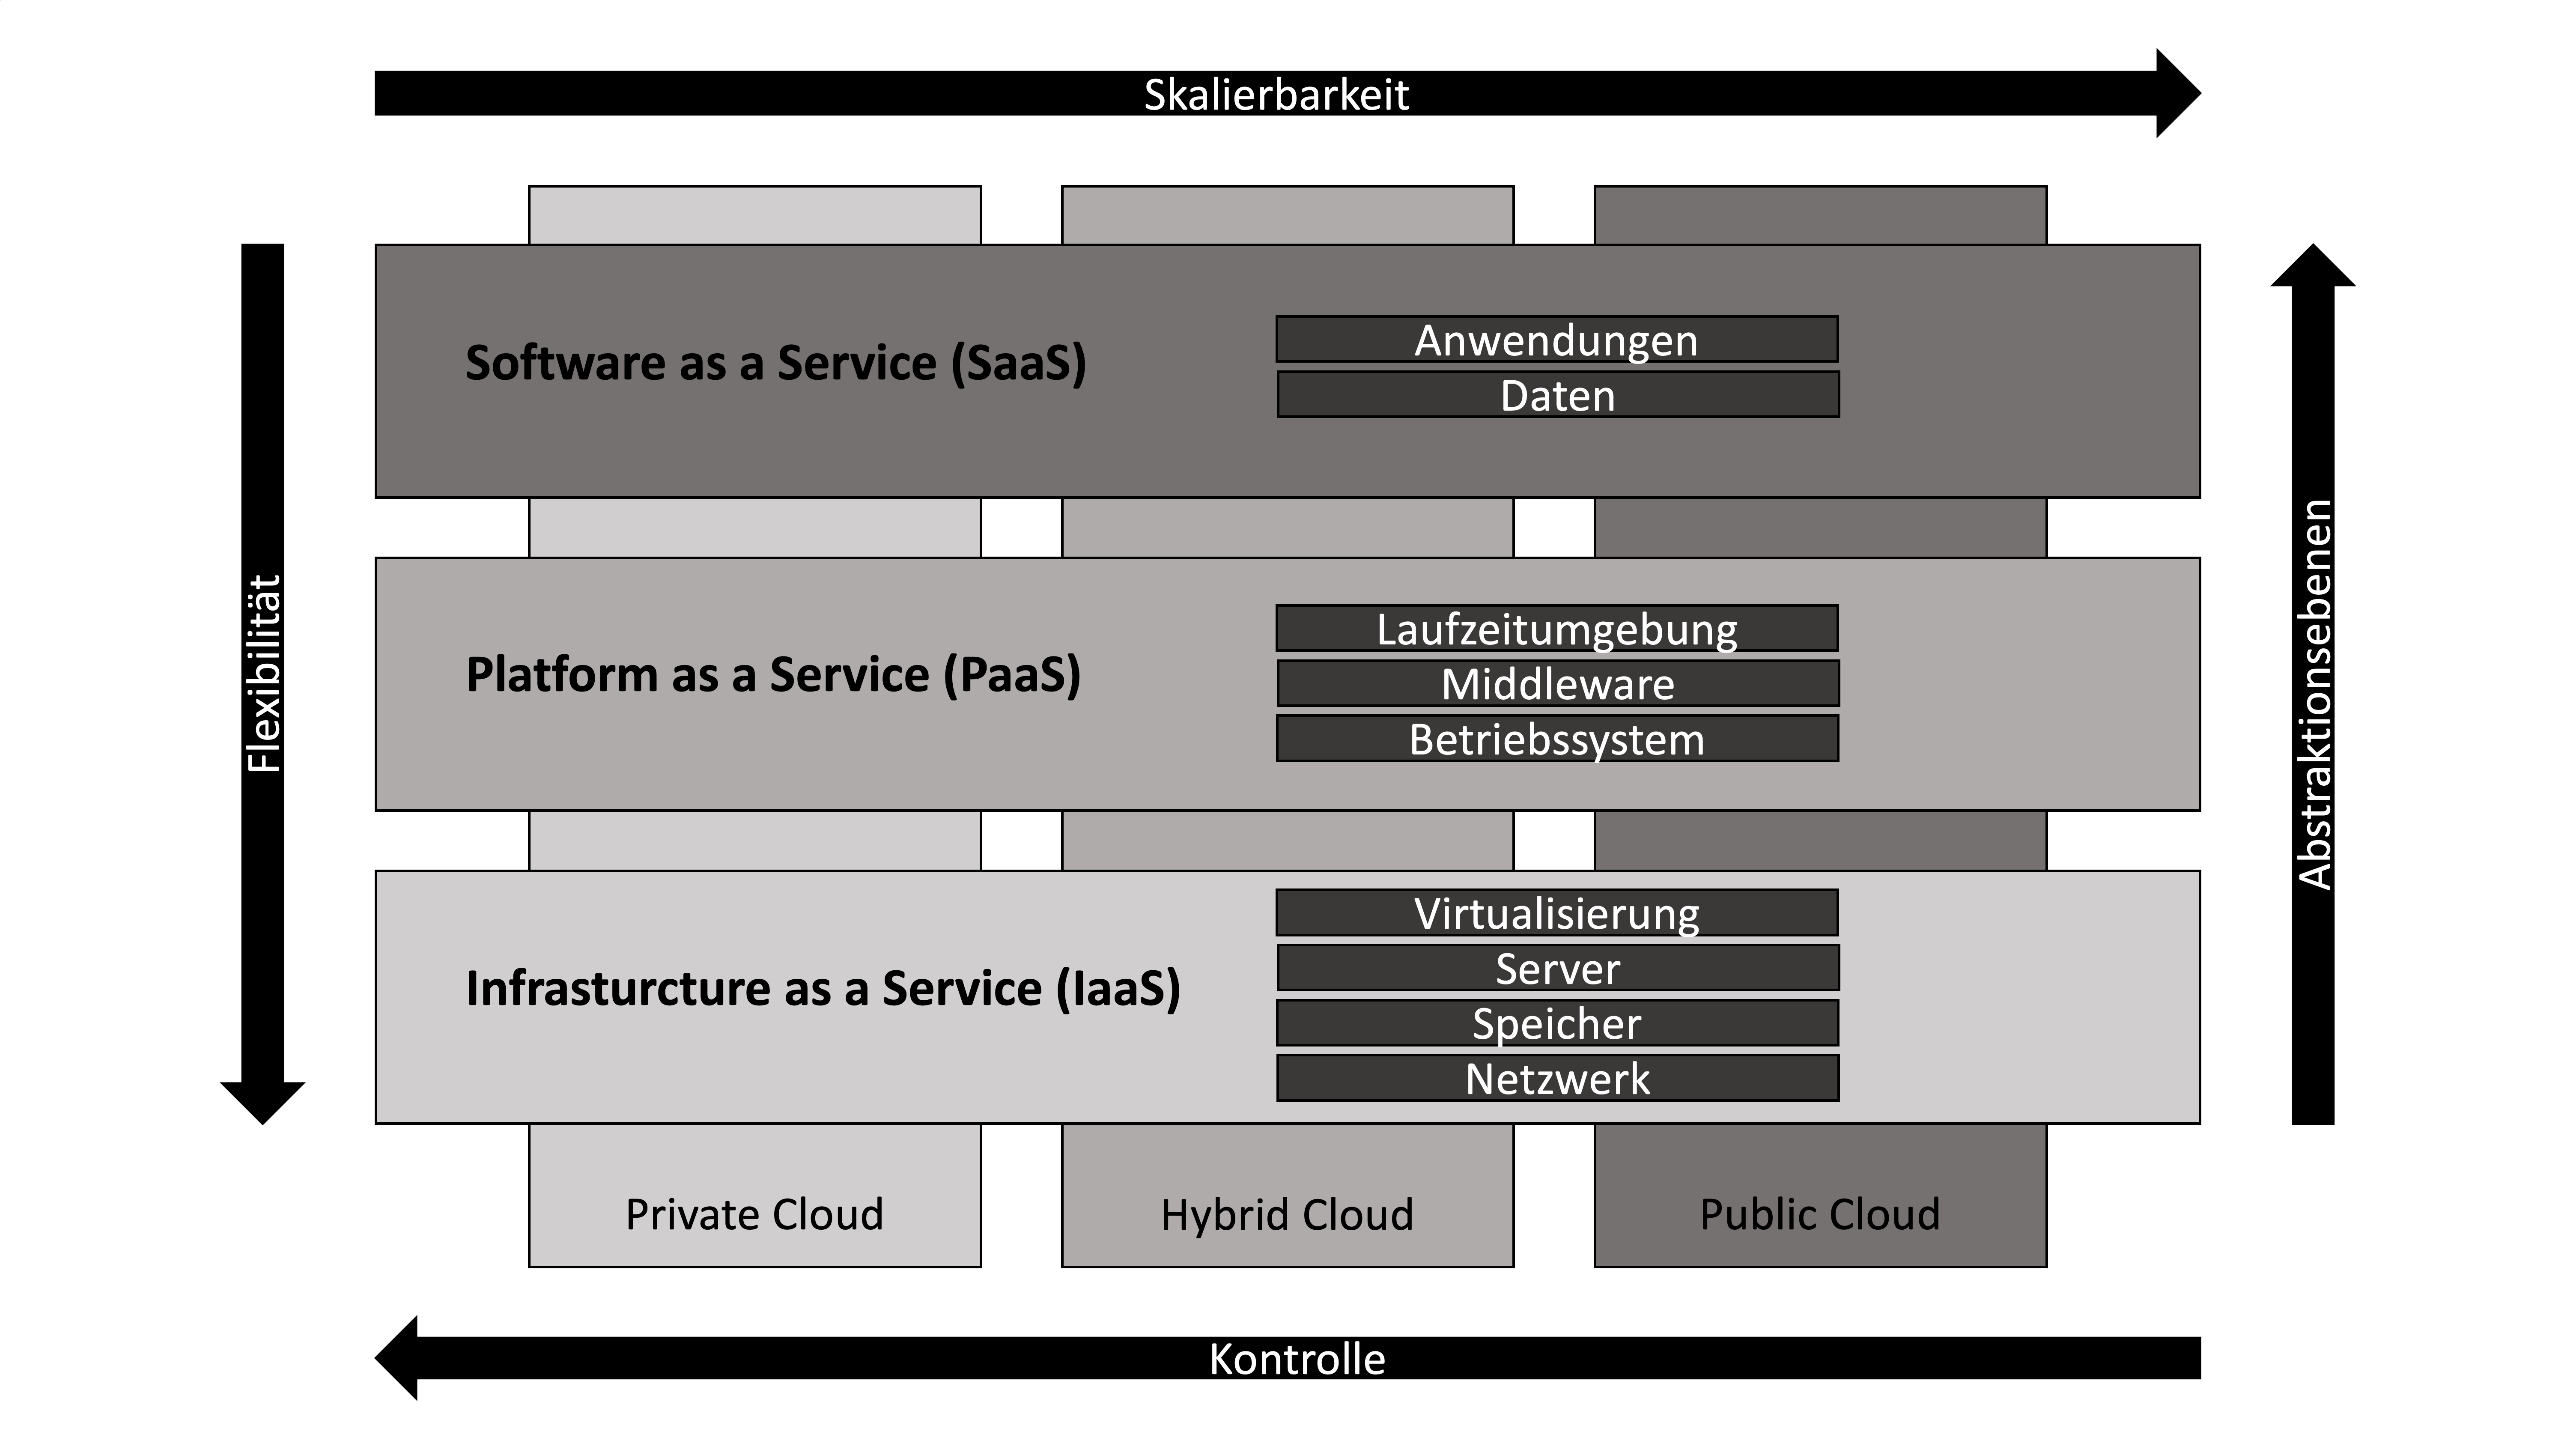
\includegraphics[height=0.3\textwidth]{xaas.png}
\caption{Eine Übersicht der Cloud Service Modelle \cite[Eigene Darstellung nach][S. 33]{Maenhaut2016}\cite[Ergänzt durch][]{Toroman2018}}
\label{fig:XaaS}
\end{wrapfigure}

Nach Hentschel und Leyh (2018), Zhao (2014), Maenhaut (2016) und Surianarayanan (2019) kann man Cloud Services grundsätzlich in drei Abstraktionsebenen einteilen. Diese sind \textbf{\ac{SaaS}}, \textbf{\ac{PaaS}} und \textbf{\ac{IaaS}}, welche auch zu \ac{XaaS} zusammengefasst werden \cite[Vgl.][S. 9]{Reinheimer2018}\cite[Vgl.][S. 143f]{Zhao2014}\cite[Vgl.][S. 32ff]{Maenhaut2016} und \cite[Vgl.][S. 226ff]{Surianarayanan2019}.

Die in Abbildung \ref{fig:XaaS} dargestellte unterste der drei genannten Abstraktionsschichten ist \ac{IaaS}, welche die Basisinfrastruktur, wie zum Beispiel Netzwerk, Server oder Speicher, bereitstellt.

Diese Infrastruktur kann sowohl physisch als auch virtuell zur Verfügung gestellt werden \cite[Vgl.][S. 9f]{Reinheimer2018}. Die darüberliegend dargestellte Schicht ist \ac{PaaS}, welche zu der Infrastrukturebene zusätzlich noch eine Basis zur Anwendungsentwicklung bietet, indem zum Beispiel bereits ein Betriebssystem und Middleware und eine Laufzeitumgebung bereitgestellt werden \cite[Vgl.][S. 10]{Reinheimer2018}. Die oberste Abstraktionsebene ist \ac{SaaS}, welche standardisierte Anwendungen zur Verfügung stellt und sich somit direkt an den Endnutzer richtet und ohne Verwaltung der zugrundeliegenden Ressourcen genutzt werden kann. Diese wird vom Provider übernommen.
\cite[Vgl.][S. 11]{Reinheimer2018}.

Generell wird die Cloud darüber hinaus in drei Organisationsdimensionen eingeteilt \cite[Vgl. auch im Folgenden][S. 7ff]{Reinheimer2018}:
\begin{itemize}
\item \textbf{Private Cloud:} Die Private Cloud bietet die exklusive Nutzung durch eine Organisation der darunterliegenden Infrastruktur. Die IT-Infrastruktur einer Private Cloud kann entweder im Unternehmenseigenen Rechenzentrum untergebracht oder auch von Dienstleistern bereitgestellt werden.
\item \textbf{Public Cloud:} In der Public Cloud ist die Infrastruktur für mehr Anwender zugänglich und muss geteilt werden. Dafür muss als Anwender oft auch nur für die tatsächlich genutzte Leistung gezahlt werden. Da die Infrastruktur jedoch gleichzeitig von vielen genutzt wird, ist zum Beispiel der Betrieb von sicherheitskritischen Anwendungen schwierig.
\item \textbf{Hybrid Cloud:} Die Hybrid Cloud bildet eine kombinierte Anwendung aus der Public Cloud und der Private Cloud. Diese bietet dem Anwender die Möglichkeit gewisse Anwendungen in die Public Cloud auszulagern, ohne die Vorteile der Private Cloud für sicherheitsrelevante Anwendungen aufgeben zu müssen. Darüber hinaus kann bei einem Hybrid Cloud Modell die Rechenleistung der Private Cloud bei Spitzenlast durch die Public Cloud erweitert werden. 
\end{itemize}

\pagebreak

\subsection{Entwicklung des Cloud Computing}

Die Entwicklung des Cloud Computing und dessen Vorgängerkonzepte is bis in die 90er Jahre zurückzuführen. Ein von Hentschel und Leyh (2018) hervorgehobener Vorgänger ist das sogenannte Grid Computing. Damit war bereits eine dezentrale Ressourcenkontrolle mir standardisierten Protokollen und Schnittstellen realisiert. Das Cloud Computing bietet vergleichbare Eigenschaften, jedoch rückt der Fokus hier auf wirtschaftliche Kriterien und die Zentralisierung von Ressourcen zum Beispiel in Rechenzentren \cite[Vgl.][S. 5f]{Reinheimer2018}.

Salesforce war eines der ersten Unternehmen, welches 1999 Anwendungen über eine Webseite bereitgestellt hat, gefolgt von den \ac{AWS} in 2002, welche Speicher und Rechenleistung als Services bereitstellten \cite[Vgl.][S. 17f]{Srivastava2018}.

\begin{figure}[h]
    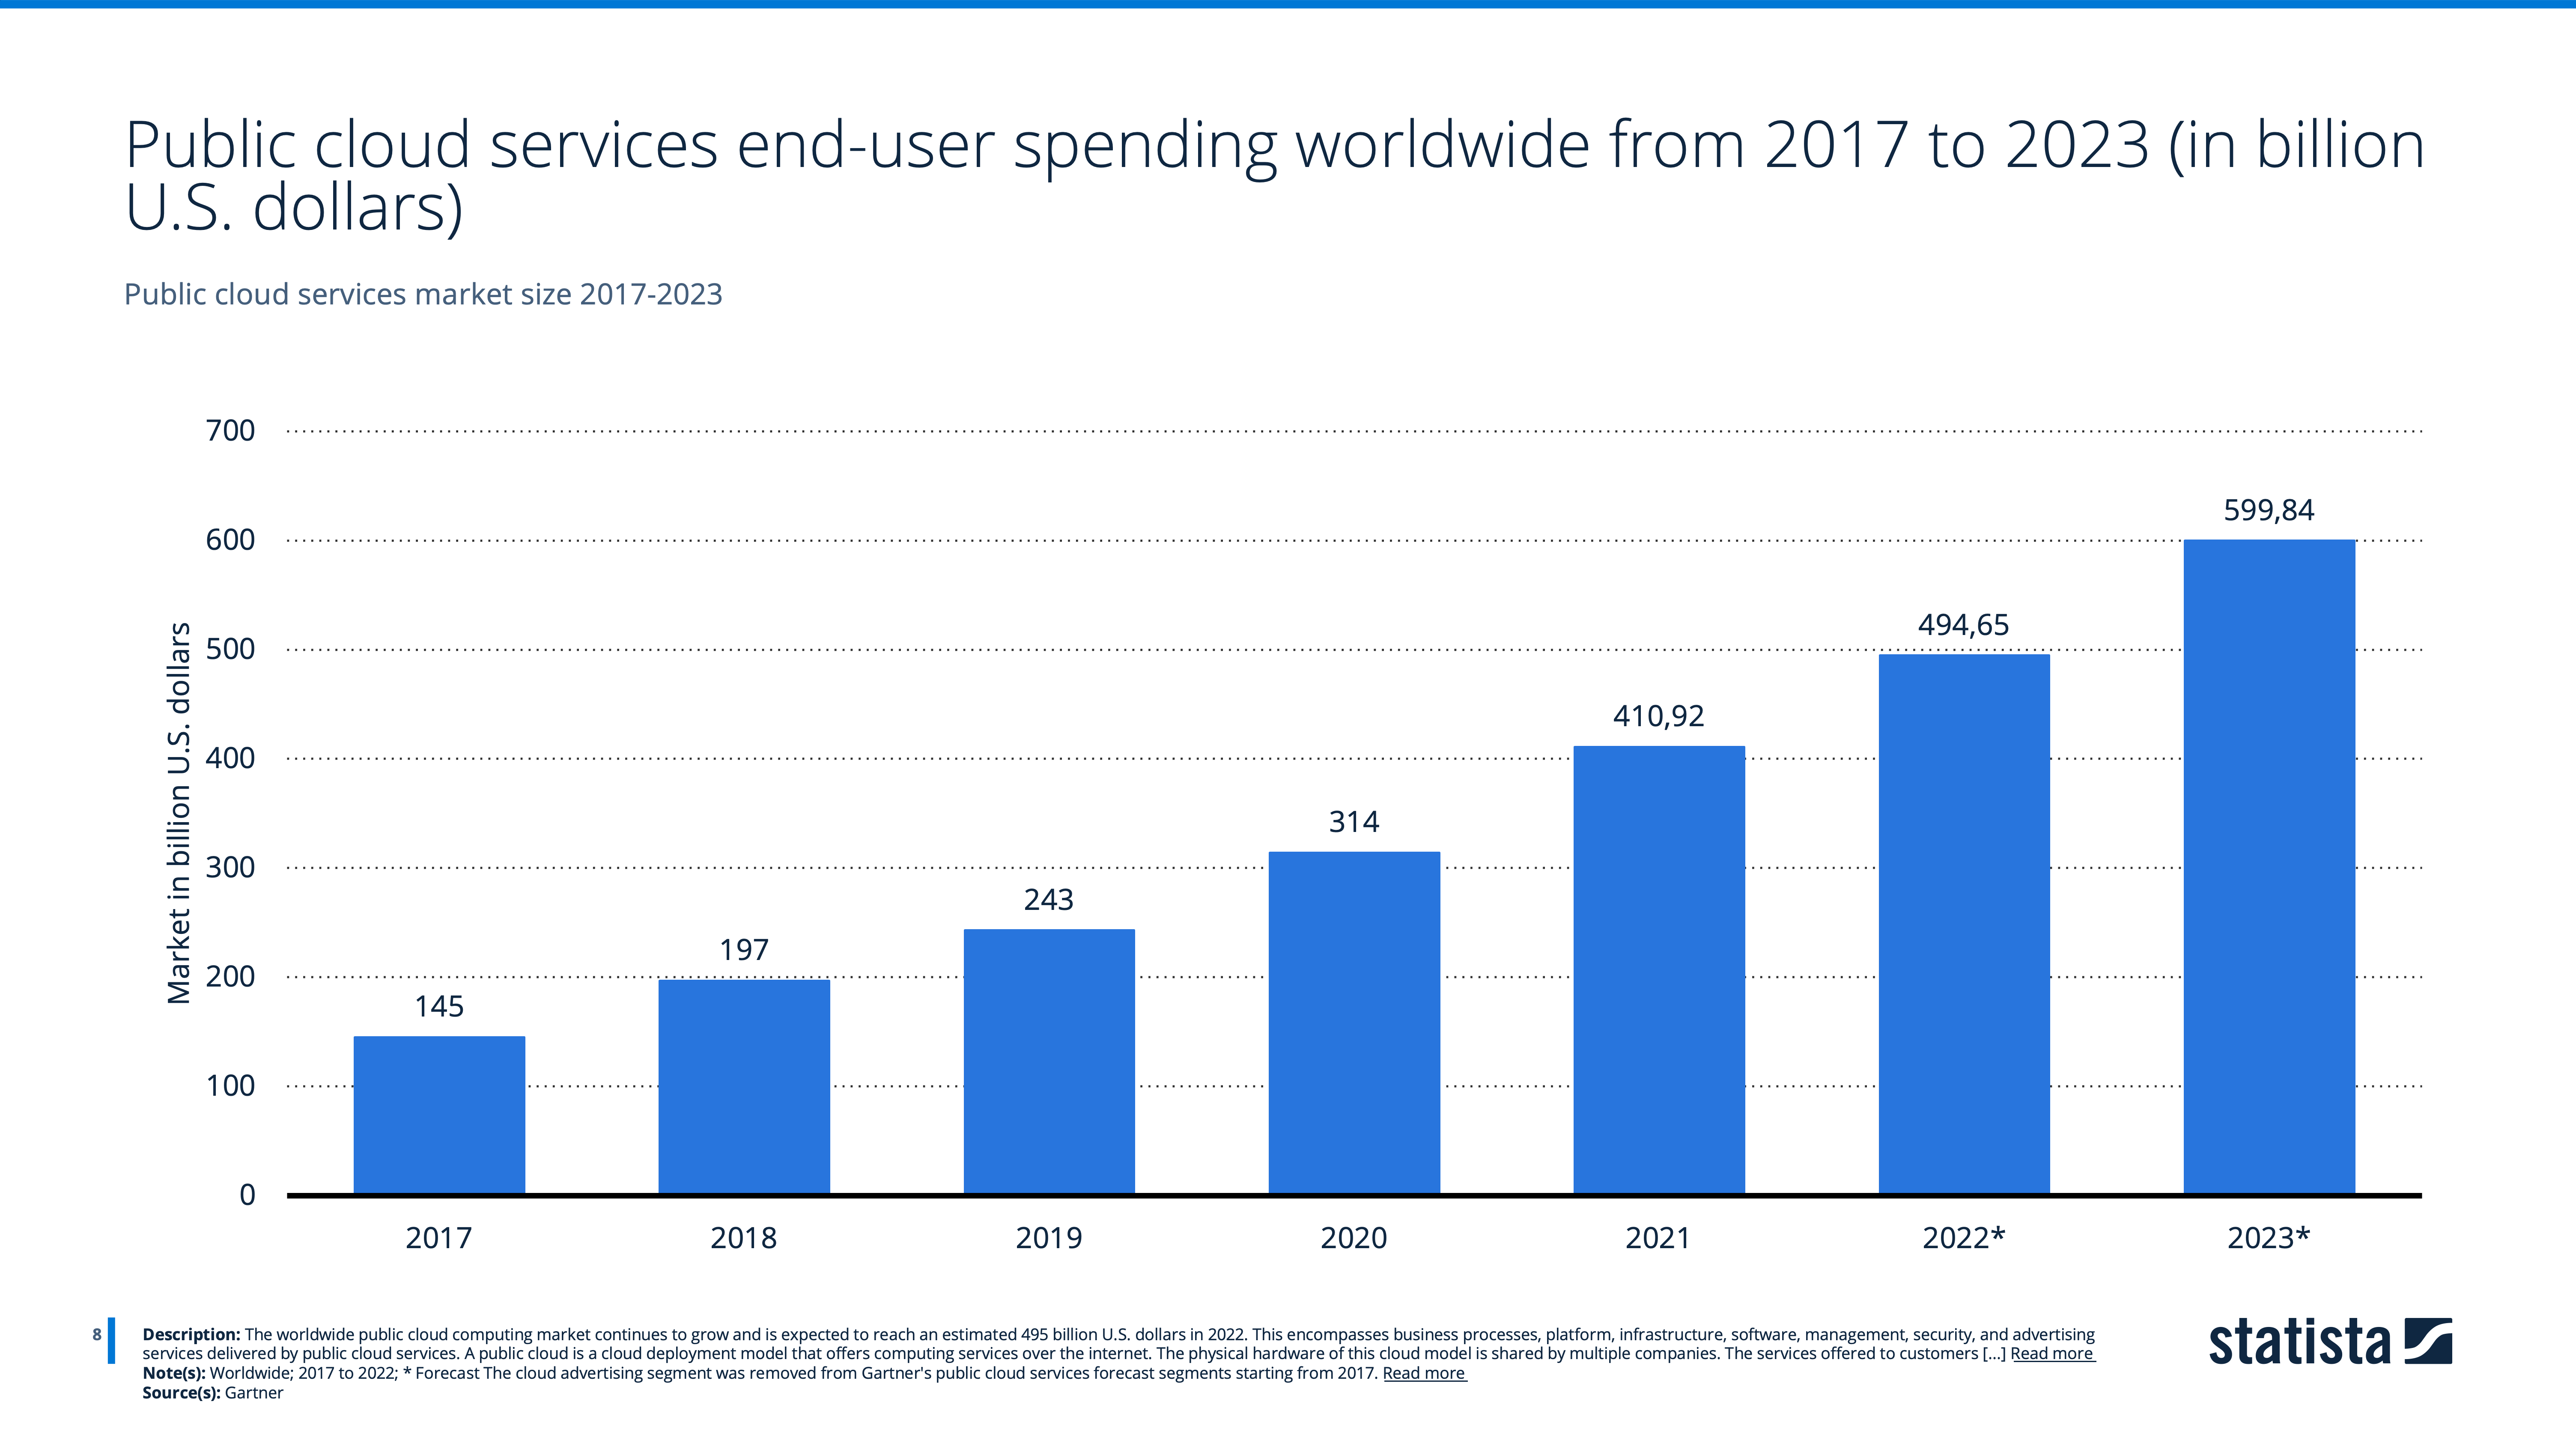
\includegraphics[width=\textwidth]{public_cloud_spending.png}
    \caption{Die Verkaufsleistungen der Public Cloud in den letzten Jahren \cite[S. 8]{Statista2022}}
    \label{fig:public_cloud_spending}
\end{figure}

Aus einem Dossier von Statista 2022 geht in der in Abbildung \ref{fig:public_cloud_spending} gezeigten Statistik hervor, dass sich die Ausgaben für public Cloud Services von 2017 bis 2023 etwas mehr als vervierfacht haben werden \cite[Vgl.][S. 8]{Statista2022}. Auch weitere Statistiken desselben Dossiers machen einen stetig steigenden Trend hinsichtlich des Cloud Computing deutlich \cite[Vgl. unter anderem][S. 11ff]{Statista2022}. 

\pagebreak

\subsection{Herausforderungen -> Migration von Legacy Anwendungen}

Neben der steigenden Nutzung von Cloud Computing und der Entwicklung Cloud basierter Anwendungen können auch legacy Anwendungen von Cloud Computing profitieren, woraus sich der trend abzeichnet, dass auch solche Anwendungen auf eine Cloud Infrastruktur migriert werden um die Ressourcen dieser nutzen zu können und Kosten zu sparen \cite[Vgl.][S. 31]{Maenhaut2016}.
\section{Merkmale von Cloud-Nativen Anwendungen}
\label{sec:cloud-native-anwendungen}
Mit Cloud-nativen Anwendungen kann das maximale Potenzial des Cloud Computing ausgenutzt werden \cite[Vgl.][]{VMwareb}. So können Produktivität und Effizienz gesteigert die Anwendungen schneller ausgeliefert werden \cite[Vgl][S. 12]{Chandrasekaran2022}. Im Folgenden werden die Merkmale von Cloud-nativen Anwendungen genauer untersucht.

% Was ist eine Cloud Native Anwendung?
% Merkmale
\subsection{Skalierbarkeit}
Von \textit{Cloud-native} Anwendungen wird unter anderem erwartet, dass diese schnell skalieren können, um unter anderem einer steigenden Nutzerzahl gerecht zu werden \cite[Vgl.][S. 1ff]{Armbrust2009} \cite[Vgl.][S. 234]{Villamizar2017}. Um die Vorteile der Cloud aber auch hinsichtlich der Kosten nutzen zu können, müssen die Services genauso herunter zu skalieren sein \cite[Vgl.][S. 884]{Adzic2017}.

Skalierbarkeit bedeutet in diesem Zusammenhang, dass die bereitgestellten IT-Ressourcen, wie Rechen- oder Speicherkapazität an die aktuelle Last angepasst werden können und entsprechen erhöht oder oder reduziert werden \cite[Vgl.][S. 15]{Reinheimer2018}\cite[Vgl.][]{Geißler2019}. Dabei wird in zwei Arten der Skalierung eines Systems unterschieden: \textbf{vertikale Skalierung} und \textbf{horizontale Skalierung} \cite[Vgl.][]{Geißler2019}\cite[Vgl.][]{VMware}

\begin{figure}[H]
    \centering
    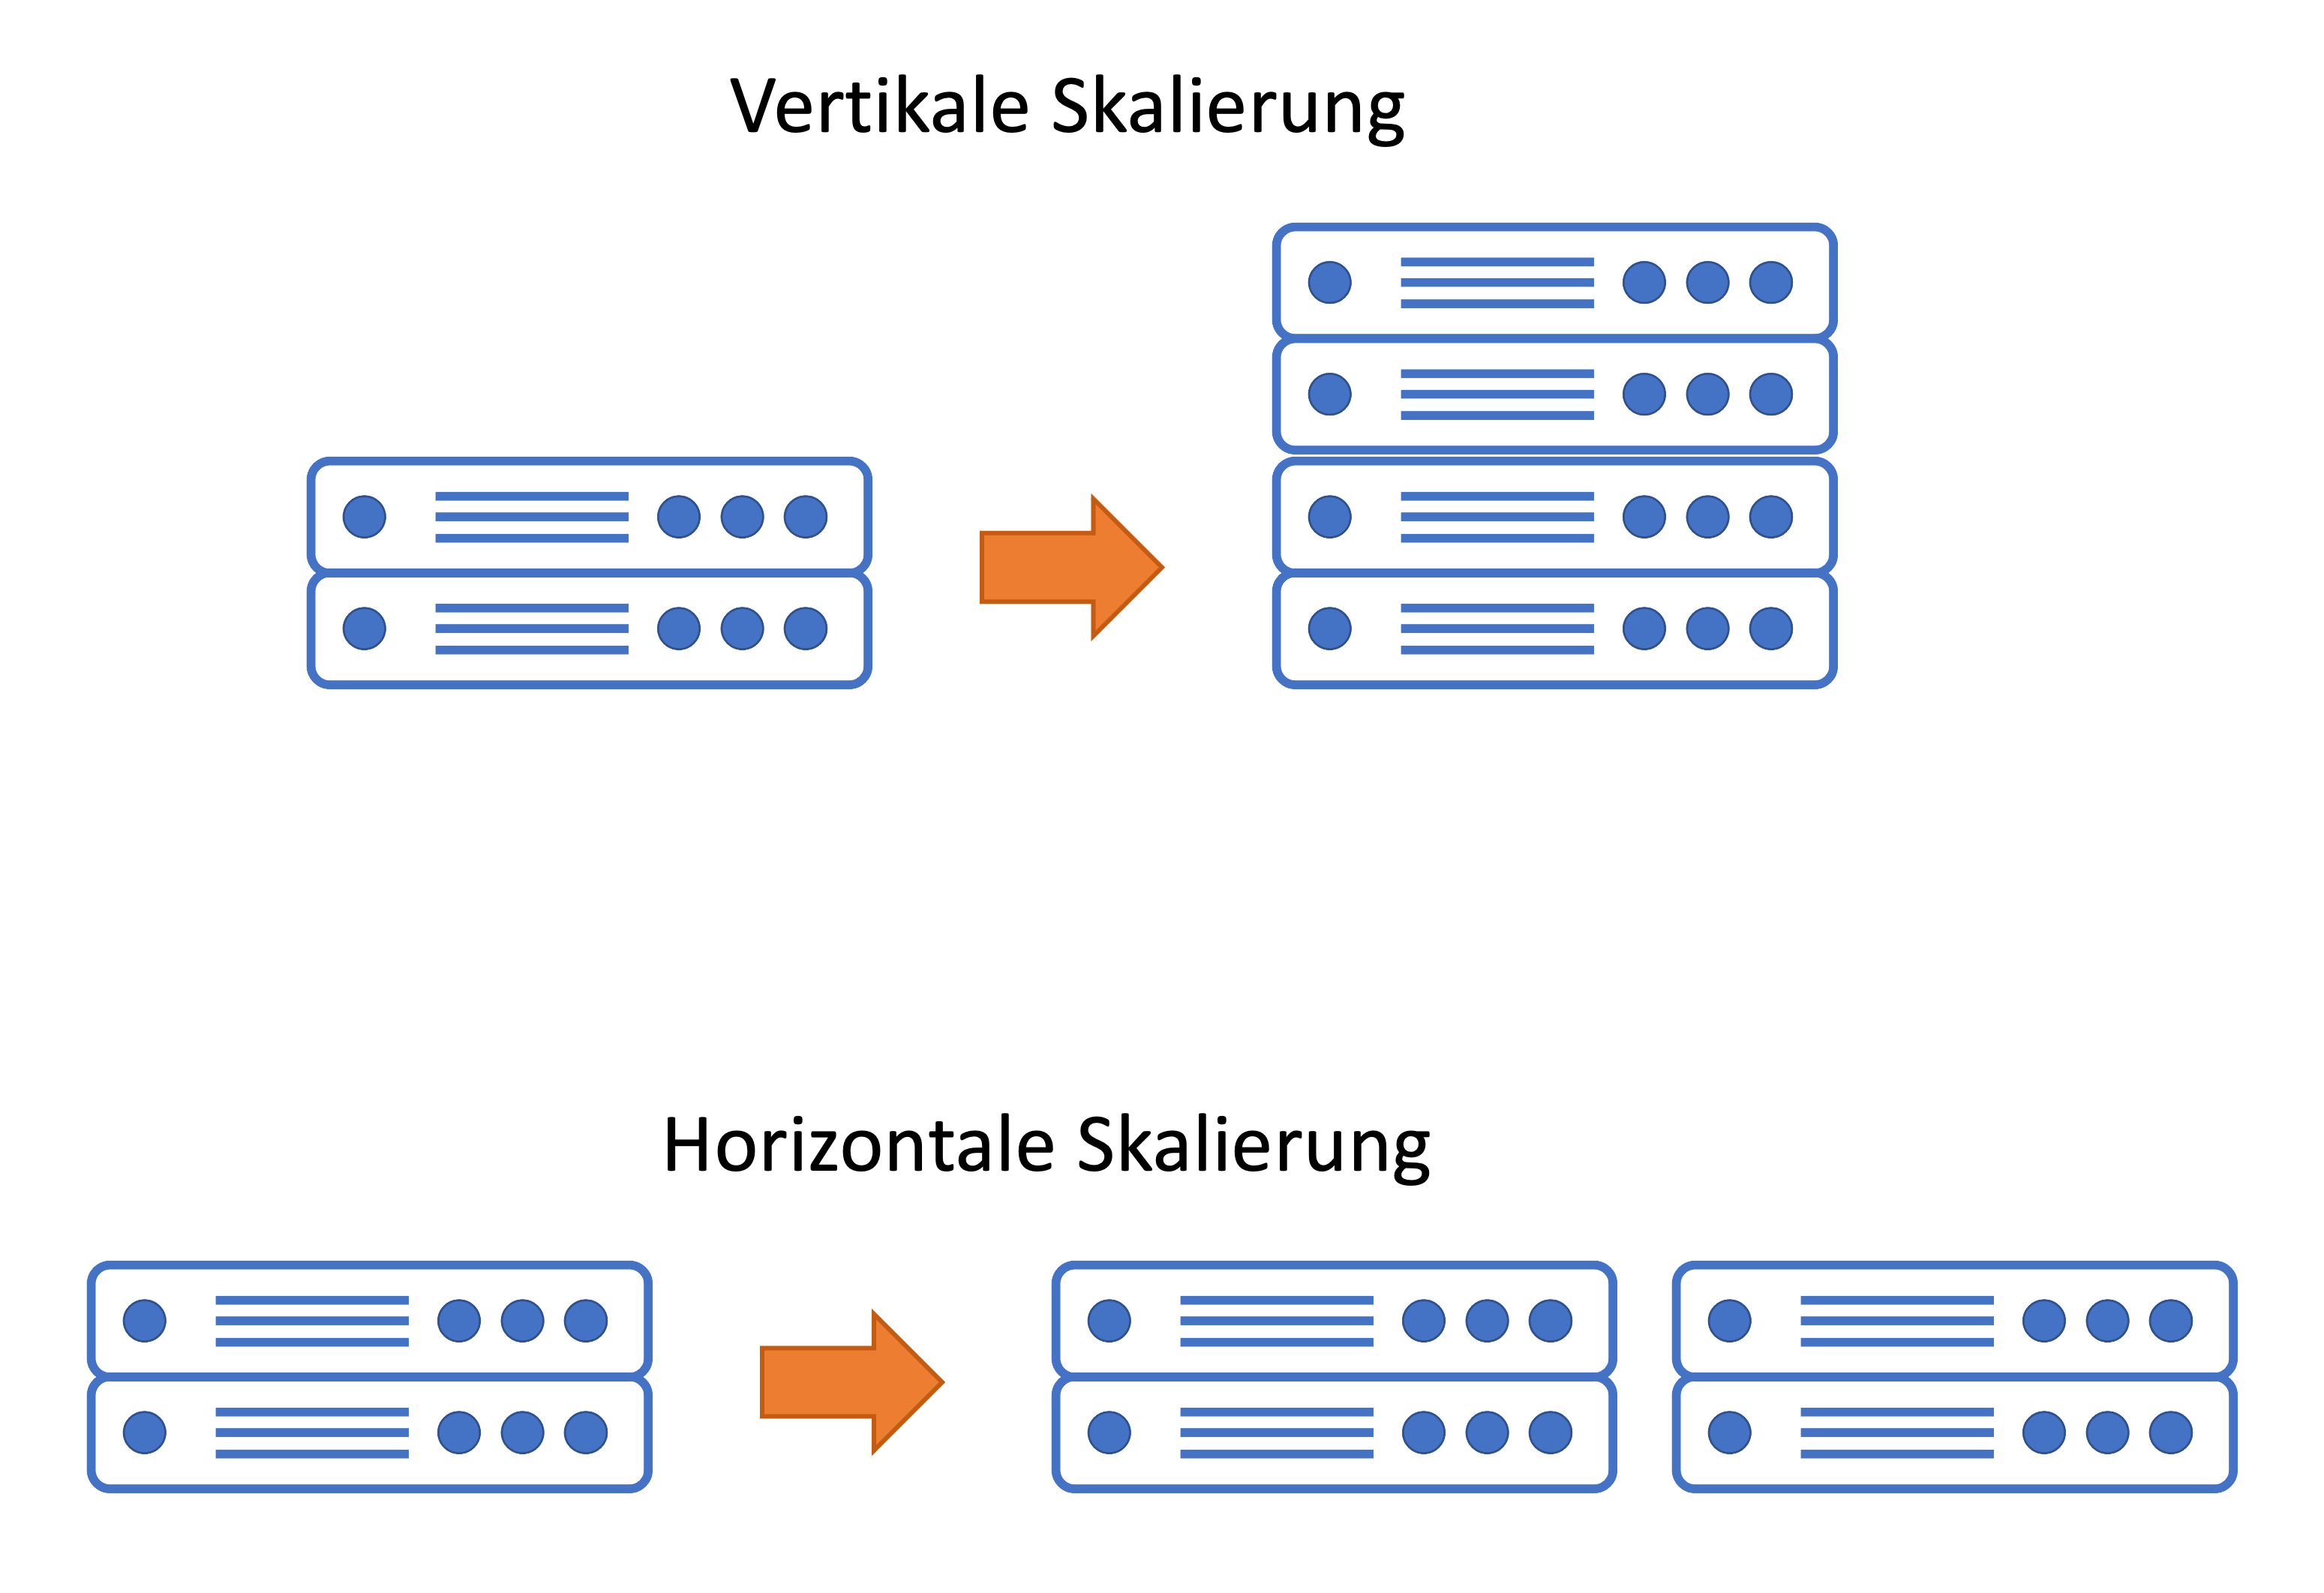
\includegraphics[width=0.65\textwidth]{scale-up_scale-out.png}
    \caption{Vertikale vs. Horizontale Skalierung \cite[Nachbildung nach][]{Bachmann2019}}
    \label{fig:scale-up-scale-out}
\end{figure}

\textbf{Vertikale Skalierung:}
Bei der vertikalen Skalierung wird zu einer Einheit innerhalb eines Systems zusätzliche Rechenleistung oder zusätzlicher Speicher hinzugefügt. Diese Art der Skalierung wird auch als ''Scale-up'' bezeichnet, abgeleitet von dem Erhöhen der Leistung. Die vertikale Skalierung ist jedoch dadurch limitiert, dass bei der Leistungsaufstockung hardwareseitig Grenzen gesetzt sind \cite[Vgl.][]{Geißler2019}\cite[Vgl.][]{VMware}. \pagebreak

\textbf{Horizontale Skalierung:}
Zur horizontalen Skalierung werden dagegen nicht die Ressourcen innerhalb einer Einheit erhöht, sondern weitere Einheiten beziehungsweise Knoten zu einem System hinzugefügt. Die Aufgaben werden dann auf mehreren Systemen durchgeführt, oder zum Beispiel eine Anwendung in mehreren Containern parallel ausgeführt. Horizontale Skalierung wird auch als ''Scale-out'' bezeichnet, da ein System hier in seiner Breite erweitert wird. In der Theorie sind der horizontalen Skalierung keine Grenzen gesetzt \cite[Vgl.][]{Geißler2019}\cite[Vgl.][]{VMware}.

\subsection{Fehlertoleranz}
Eine weitere Anforderung an Cloud-native Anwendungen ist die Fehlertoleranz. Es sollte grundsätzlich davon ausgegangen, dass Fehler auftreten können und diese abgefangen werden müssen \cite[Vgl.][S. 17]{Gannon2017}. Zu diesen Fehlern gehört unter anderem das Abstürzen von Container und Hardware- oder Netzwerkfehler.
% Auch durch horizontale Skalierung, weil einzelne Nodes ausfallen können

\subsection{Schnelle Bereitstellung}
Mit \textit{Continous Delivery}, zu deutsch kontinuierliche Bereitstellung, können Änderungen in der Anwendung unmittelbar ausgeliefert werden, ohne zum Beispiel auf ein Wartungsfenster nachts warten zu müssen oder die Änderungen mit weiteren Updates zu einem Release zu bündeln, bevor diese ausgeliefert werden \cite[Vgl.][]{VMwareb}.

\subsection{Containerisierung}
Gegenüber der Verwendung von \acp{VM} bieten Container eine höhere Effizienz und Geschwindigkeit. Das Starten und Beenden von Containern ist ein einer \ac{VM} zeitlich voraus. Darüber hinaus benötigt eine \ac{VM} weitere Pakete, da diese die Hardware virtualisiert, wogegen in Containern nur das Betriebssystem virtualisiert wird \cite[Vgl.][]{VMwareb}.

\subsection{Weitere Merkmale}
% Vorhersehbarkeit, kollaborative Entwicklung, Microservices
Weitere Merkmale Cloud-nativer Anwendungen sind unter anderem eine bessere Verlässlichkeit, durch eine gewährleistete ''Ausfallsicherheit'' und die Verwendung vieler unabhängiger Microservices (siehe Kapitel \ref{sec:architekturstile}), wodurch auch die Entwicklung in Teams erleichtert wird, da die Services unabhängig voneinander aktualisiert werden können \cite[Vgl.][]{VMwareb}.

\pagebreak
\section{Herausforderungen der Cloud Migration}
\label{sec:herausforderungen}

% Merkmale von Cloud nativen Anwendungen in legacy Applikationen umsetzen
% Verlass auf Box-API muss gegeben sein
% https://developers.redhat.com/articles/2021/06/14/application-modernization-patterns-apache-kafka-debezium-and-kubernetes#application_modernization_in_context

Cloud Computing birgt jedoch auch einige Herausforderungen, welche in der Entwicklung und Migration komplexe Aufgaben mit sich bringen können.

\subsection{Vorteile der Cloud nutzen}

Neben der steigenden Nutzung von Cloud Computing und der Entwicklung Cloud-basierter Anwendungen können auch \textit{legacy} Anwendungen von Cloud Computing profitieren. Daraus zeichnet sich der Trend ab, dass auch solche Anwendungen auf eine Cloud Infrastruktur migriert werden. Diese Entwicklung ermöglicht es, die Ressourcen der Cloud nutzen zu können und Kosten zu sparen \cite[Vgl.][S. 31]{Maenhaut2016}.

Abhängig vom gewählten Migrationsansatz sind Anpassungen in der Anwendung vorzunehmen, meist um die Vorteile der Cloud ausnutzen zu können. Verbesserung des Anwendungsdesigns und die Optimierung von Ressourcennutzung sind nach Feathers (2004) zwei der vier möglichen Hauptgründe Anpassungen an Software vorzunehmen \cite[Vgl.][S. 3]{Feathers2004}. Diese lassen sich auch auf die vorzunehmenden Anpassungen für eine Cloud Migration übertragen. Eine Herausforderung, die bei der Anpassung von Software aufkommt, ist es sicherzustellen das grundlegende Verhalten der Anwendungen nicht zu beeinträchtigen. Die Schwierigkeit liegt darin, oft nicht genau erkennen zu können, wie Stark das Verhalten der Anwendung auf diese Änderungen reagiert \cite[Vgl.][S. 7]{Feathers2004}. 

\subsection{Entwicklung von Cloud-basierten Anwendungen}

Eine weitere Herausforderung in der Anwendungsentwicklung ist, die Anwendung und den Entwicklungsprozess so zu gestalten, dass mehrere Entwickler gleichzeitig an verschiedenen Funktionen der Anwendung arbeiten können, ohne sich dabei gegenseitig in die Quere zu kommen. Auch darauf ist entsprechend bei der Cloud Migration von \textit{legacy} Anwendungen zu achten \cite[Vgl.][]{Ibryam2021}.

Außerdem wird im Zuge der Migration meist erwartet, dass die Vorteile der Cloud, wie zum Beispiel eine effiziente Skalierung der Anwendung, umgesetzt werden, was zusätzlichen Aufwand zur reinen Migration bedeutet \cite[Vgl.][]{Ibryam2021}. \pagebreak

\subsection{Datenschutz und Datensicherheit in der Cloud}
Personenbezogene und sensible (z. B. geschäftliche) Daten bedürfen einer guten Datensicherheit, vor allem im Kontext des Cloud Computing und dort insbesondere für die Public Cloud, wo Speicherressourcen nicht direkt in den Händen des Anwenders liegen, sondern in den Rechenzentren der Provider verarbeitet und gespeichert werden \cite[Vgl.][S. 1ff]{Sun2019}. Aus diesem Grund ist es wichtig, mögliche Risiken sowie die damit verbundenen Herausforderungen zu identifizieren \cite[Vgl.][S. 3]{Sun2019}.

Folgende Risiken können für Datenschutz und Datensicherheit in der Cloud existieren \cite[Vgl. auch im folgenden][S. 694]{Kumar2018}:

\begin{itemize}
    \item Risiken in Zusammenhang mit \textit{\ac{CIA}}\footnote{dt. Konsistenz, Integrität und Verfügbarkeit, }
    \item Herausforderungen bei der Authentifizierungs- und Zugriffskontrolle
    \item Fehlerhafte Authentifizierungs-, Sitzungs- und Zugriffskontrollen
    \item Weitere Risiken, die durch z. B. Speicherort der Daten, Mehrbenutzerfähigkeit oder Backups entstehen können
\end{itemize}

\pagebreak
\section{Migrationsansätze}
\label{sec:migrationsansaetze}

Im folgenden Kapitel wird auf die unterschiedlichen Migrationsmethoden des Cloud Computing eingegangen. Durch die unterschiedlichen Abstraktionsebenen bedingt gibt es verschiedene Ansätze, wie die Cloud Migration realisierbar ist \cite[Vgl.][S. 226]{Surianarayanan2019}, angefangen mit dem auch als \glqq{Lift and Shift}\grqq{} bezeichneten Rehosting, bis hin zur Migration zu \ac{SaaS} verbunden mit der Entwicklung Cloud nativer Anwendungen \cite[Vgl.][S. 144]{Zhao2014}.

\subsection{Migration zu IaaS (Rehosting)}
Nach Zhao (2014) ist vorallem das Rehosting die vorgeschlagene Strategie für die Migration zu \ac{IaaS} \cite[Vgl.][S. 144]{Zhao2014}. Umgangssprachlich wird diese Vorgehensweise auch als \glqq{Lift and Shift}\grqq{} bezeichnet \cite[Vgl.][]{NetApp}. Bei diesen Strategien werden Anwendungen lediglich auf einer anderen Hardwareplattform installiert, die Anwendungsarchitektur bleibt dabei unverändert. Dieser Ansatz bietet eine schnelle Lösung zur Migration \cite[Vgl.][]{CIO}.

Der wahrscheinlich größte Vorteil der Migration zu \ac{IaaS} ist, dass die Anwendungsarchitektur nicht verändert werden muss und die Migration somit schnell und ohne großen Aufwand vollzogen werden kann. Ein Nachteil ist dagegen, dass die Migration zu \ac{IaaS} nicht die vollen Möglichkeiten der Cloud ausnutzt.

\subsection{Migration zu PaaS (Refactoring/Rebuilding)}
Das Refactoring oder Rebuilding von Anwendungen gehört nach Zhao (2014) zu den empfohlenen Strategien für die Migration zu \ac{PaaS} \cite[Vgl.][S. 144]{Zhao2014}. Rebuilding bedeutet, den bisherigen Code zu re-architekten um die Vorteile der Cloud Plattform nutzen zu können \cite[Vgl.][]{CIO}. Darunter fällt zum Beispiel das Umsetzen entsprechender Service Topologien im Code \cite[Vgl.][S. 2]{Holmes2018}.

Durch die vom Cloud Provider teils vorgegebene Plattform (z.B. Middleware und Datenbanken) müssen Anwendungen dieser entsprechend angepasst werden \cite[Vgl.][S. 227]{Surianarayanan2019}. Der Mehrwert einer Migration zu \ac{PaaS} ist, dass der Anwender die IT-Infrastruktur nicht mehr managen muss und somit Aufwände reduziert werden können \cite[Vgl.][S. 6]{Pahl}.

\subsection{Migration zu SaaS (Cloud Native Entwicklung)}
Der Schritt zu \ac{SaaS} ist nach Zhao (2014) auf verschiedenen Wegen zu erreichen. Demnach sei eine Anwendung durch einen SaaS Service entweder zu ersetzen, entsprechend der SaaS Prinzipien zu überarbeiten oder zu einem \ac{SaaS} Service umzustrukturieren \cite[Vgl.][S. 144]{Zhao2014}.

Das Augeben einer Anwendung und vollständige Ersetzen dieser durch Nutzung des \ac{SaaS} Modells bedarf eines größeren Aufwand und ein Entwicklungsteam zur Umsetzung der Anforderungen \cite[Vgl.][]{CIO}.
\section{Architekturstile im Hintergrund des Cloud Computing}
\label{sec:architekturstile}
Die Architektur von Anwendungen ist in den meisten Fällen entweder monolithisch oder als Microservice Architektur umgesetzt \cite[Vgl.][S. 150]{Gos2020}. Das nachfolgende Kapitel beschreibt diese Architekturstile mit ihren Eigenschaften und aus welchem Grund die Microservice Architektur für den Betrieb in der Cloud bevorzugt eingesetzt wird \cite[Vgl.][S. 1]{Villamizar2015}.

\subsection{Monolithische Anwendungsarchitektur}
% Was sind monolithische Anwendungen?
Monolithische Anwendungen, wie sie in der Vergangenheit oft eingesetzt wurden, bestehen aus verschiedenen Komponenten, die zu einem Programm kombiniert werden. Die einzelnen Komponenten funktionieren nur zusammen innerhalb des Monolithen, einzelne Komponenten können also nicht unabhängig betrieben werden. \cite[Vgl.][S. 1]{Gos2020}.

\begin{figure}[H]
    \centering
    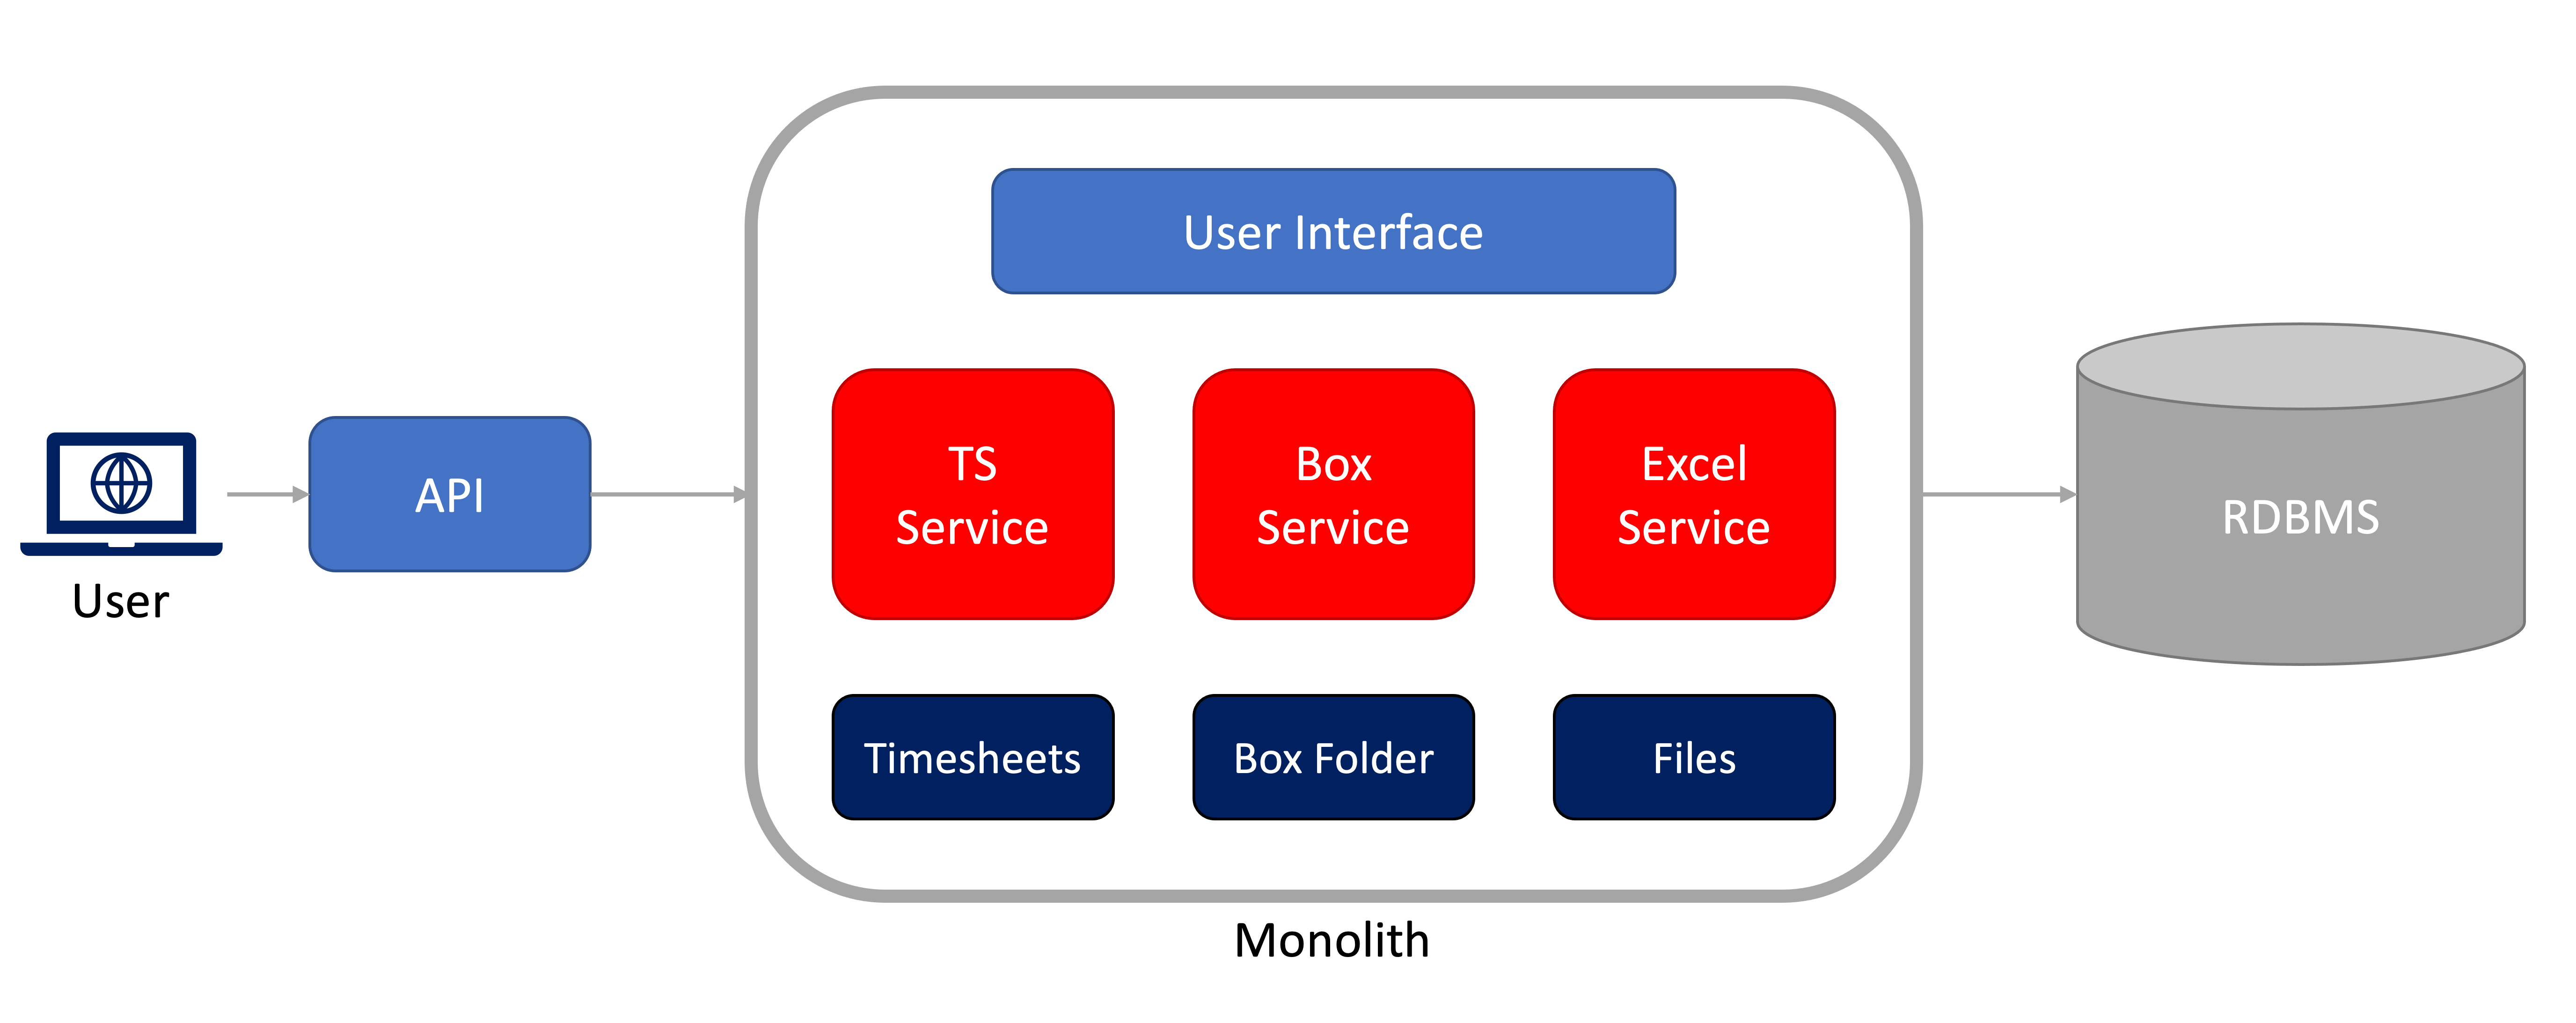
\includegraphics[width=0.65\textwidth]{monolith.png}
    \caption{Beispiel einer monolithischen Architektur \cite[Nachbildung angelehnt an][S. 150]{Gos2020}}
    \label{fig:monolith}
\end{figure}

Abbildung \ref{fig:monolith} zeigt, wie eine monolithische Architektur aufgebaut sein kann. Hier sind die Komponenten eng miteinander verwoben und voneinander abhängig.
% In Bezug auf Cloud Native -> warum nicht geeignet
\pagebreak

\subsection{Microservice Architektur}
Der Einsatz von Microservice Architekturen hat in den letzten Jahren stark zugenommen \cite[Vgl.][S. 150]{Gos2020}. Microservices bedeutet, dass eine Anwendung aus einer Zusammenstellung einzelner Services besteht, wobei jeder Service einen Teil der Business-Logik erfüllt. Diese Services sind dabei, wie in Abbildung \ref{fig:microservice} dargestellt voneinander unabhängig um keinen Single-Point of Failure zu erzeugen \cite[Vgl.][S. 150]{Gos2020}\cite[Vgl.][]{Janssen2021}\cite[Vgl.][]{Fowler2014}.

\begin{figure}[H]
    \centering
    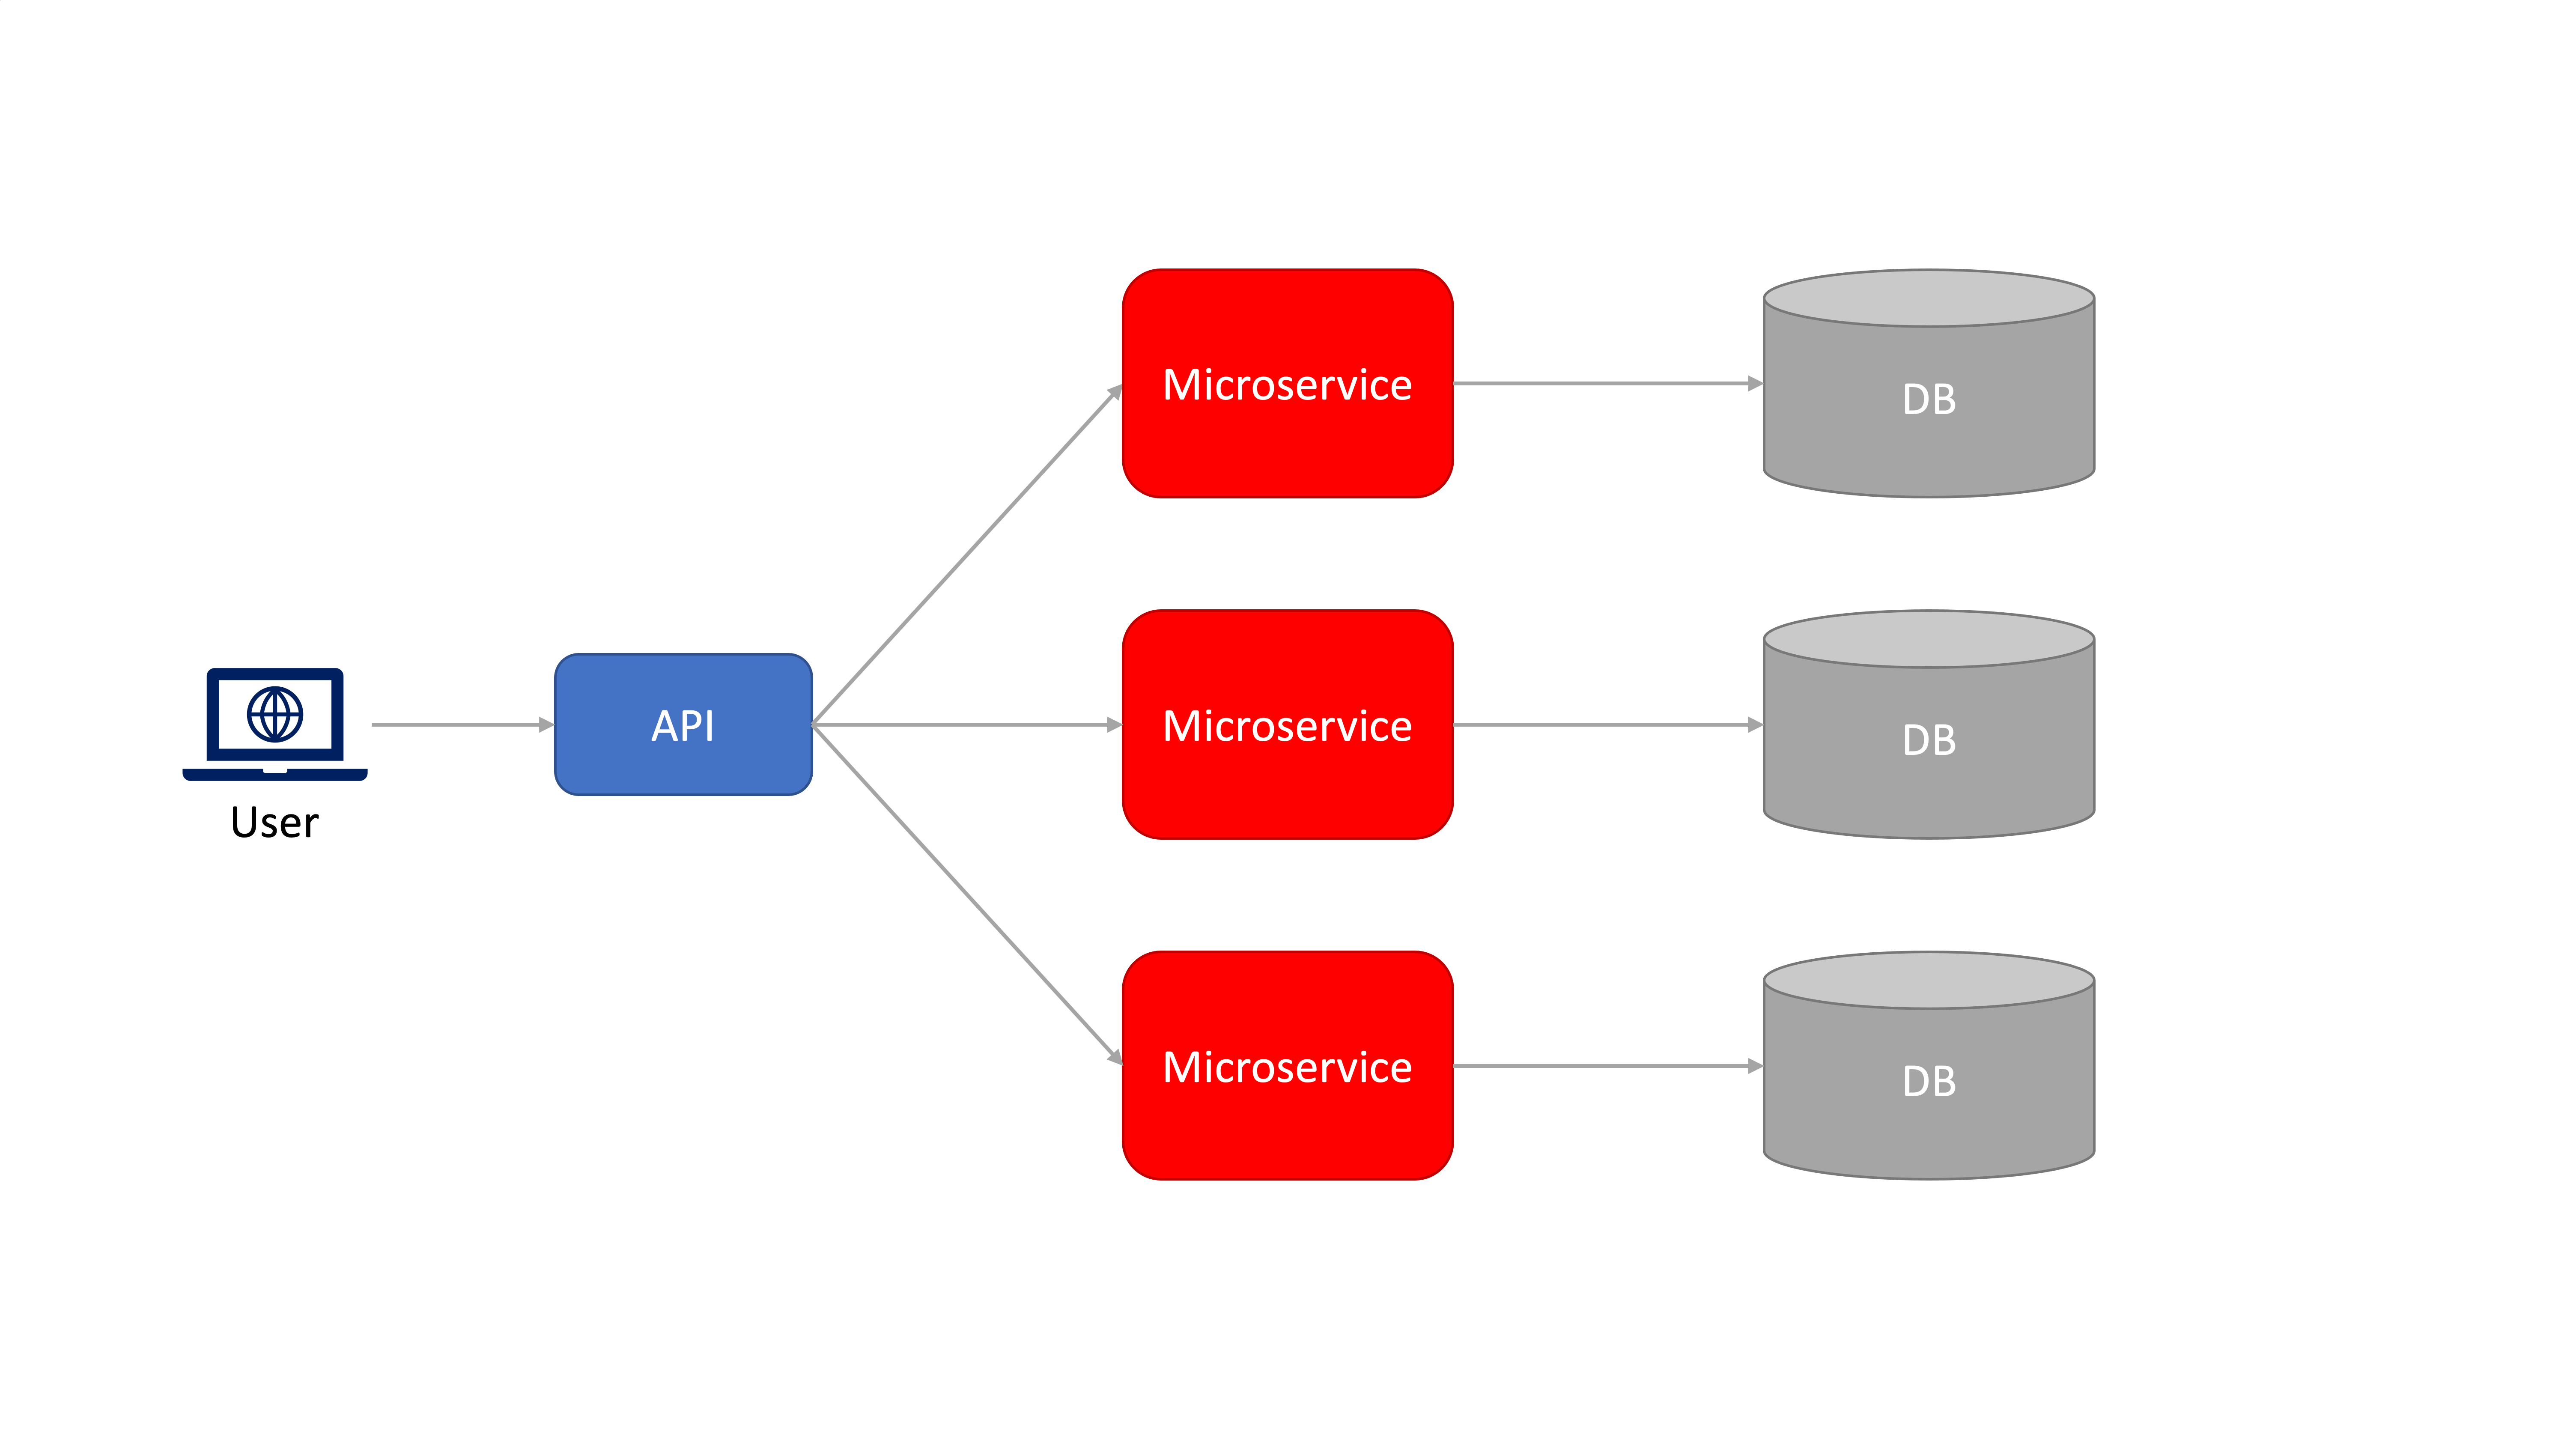
\includegraphics[width=0.65\textwidth]{microservice.png}
    \caption{Beispiel einer Microservice Architektur \cite[Nachbildung angelehnt an][S. 150]{Gos2020}}
    \label{fig:microservice}
\end{figure}

In Bezug auf Cloud-native Anwendungen bringen Microservices eine effizientere Skalierbarkeit mit sich, da jeder Service einzeln je nach Bedarf skaliert werden kann und nicht die komplette monolithische Anwendung skaliert werden muss \cite[Vgl.][]{Janssen2021}.

Die Entwicklung von Microservices hat außerdem den Vorteil, dass der Blick im Entwicklungsprozess separiert auf die einzelnen Services gelegt werden kann und der Entwickler somit nicht jederzeit den ganzen Monolithen im Auge haben muss, um zu verhindern, dass einzelne Funktionen sich gegenseitig beeinflussen \cite[Vgl.][]{Janssen2021}. \pagebreak

% In Bezug auf Cloud Native -> weil skalierbar (kleine Einheiten etc...)
% Fehlertoleranter
% Asynchrones Messaging (-> keine Fails, wenn Service ausfällt)
\section{Serverless Computing} % vs. Server-Aware
\label{sec:serverless-serveraware}

% \subsection{Server-Aware}
% \label{sec:server-aware}

% Der englische Begriff \textit{Server Aware} bedeutet auf deutsch, sich dem Server Bewusst sein. Bei der Nutzung von \ac{IaaS} hat der Entwickler die meiste Kontrolle über Anwendungen und die Infrastruktur in der Cloud und ist verantwortlich für die Bereitstellung von zum Beispiel Hardwareressourcen und \acp{VM} \cite[Vgl.][S. 3]{Baldini2017}.

% \subsection{Serverless}
% \label{sec:serverless}

% Beim Einsatz von \ac{PaaS} und \ac{SaaS} Service Modellen ist der Entwickler ''nichtwissend'' (\textit{unaware}) über die Cloud Infrastruktur \cite[Vgl.][S. 3]{Baldini2017}. \textit{Serverless}, also Serverlos ist eigentlich kein zutreffender Name, da die Infrastruktur und Server nach wie vor existieren, der Entwickler sich lediglich nicht darum kümmern muss, wie diese aussehen \cite[Vgl.][S. 5]{Baldini2017}.

In den vergangenen Jahren hat sich \textit{Serverless Computing} als neues Paradigma des Cloud Computing entwickelt \cite[Vgl.][S. 44]{Castro2019}\cite[Vgl.][S. 64]{Anel2020}. Mit \textit{Serverless Computing} sollen sich die Vorteile der Cloud optimal ausnutzen lassen \cite[Vgl.][S. 6]{Eivy2017}\cite[Vgl.][S. 8]{Jonas2019}. Zu diesen Vorteilen gehört unter anderem die Skalierbarkeit der Infrastruktur \cite[Vgl.][S. 1ff]{Armbrust2009}\cite[Vgl.][S. 234]{Villamizar2017}\cite[Vgl.][S. 884]{Adzic2017}.

\textit{Serverless} Computing bedeutet, dass die Entwickler unabhängig von der Cloud-Infrastruktur entwickeln können. Der Begriff wird noch besser durch den gegenteiligen Begriff \textit{Server Aware} (dt. Server-bewusst) verständlich, da dieser deutlich macht, dass Entwickler sich dabei der Server und Infrastruktur bewusst sein müssen. Bei \textit{Serverless Computing} ist dagegen keine Kenntnis über die zugrundeliegende Infrastruktur notwendig \cite[Vgl.][S. 5]{Jonas2019}\cite[Vgl.][S. 1]{Hellerstein2018}\cite[Vgl.][S. 46]{Castro2019}\cite[Vgl.][S. 64]{Anel2020}.

Darüber hinaus bringt \textit{Serverless} den Vorteil mit sich, dass eine Abrechnung der Kosten nur dann erfolgt, wenn die Anwendungen auch ausgeführt werden, da die Ressourcen nur für den Ausführungszeitraum bereitgestellt werden. Bei \textit{Server-aware} Services würde bereits die Bereitstellung diese Kosten verursachen. \cite[Vgl.][S. 46]{Castro2019}. Mit \textit{Serverless} kann die Infrastruktur effizienter genutzt werden, da diese nicht dauerhaft für bestimmte Anwendungen reserviert ist und die Produktivität in der Entwicklung steigt \cite[Vgl.][S. 9]{Jonas2019}. Da für diese automatische Skalierung und Bereitstellung der Ressourcen der Cloud Provider verantwortlich ist, kann diese für den Anwender transparent gemacht werden \cite[Vgl.][S. 47]{Castro2019}.
\pagebreak

%title wird unter dem Bsp. abgedruckt
%caption wird im Verzeichnis abgedruckt
%label wird zum referenzieren benutzt, muss einzigartig sein.

% \begin{lstlisting}[caption=Code-Beispiel, label=Bsp.1]
% public class HelloWorld {
% 	public static void main (String[] args) {
% 		// Ausgabe Hello World!
% 		System.out.println("Hello World!");
% 	}
% }
% \end{lstlisting}

% %language ändert die Sprache. (Wenn nur eine Sprache verwendet wird, kann diese Sprache in einstellungen.tex geändert werden. Standardmäßig Java.)
% \begin{lstlisting}[caption=Python-Code, label=Python-Code, title=Titel des Python-Codes,language=Python]
% def quicksort(liste):
% if len(liste) <= 1:
% 	return liste
% pivotelement = liste.pop()
% links = [element for element in liste if element < pivotelement]
% rechts = [element for element in liste if element >= pivotelement]
% return quicksort(links) + [pivotelement] + quicksort(rechts)
% # Quelle: http://de.wikipedia.org/wiki/Python_(Programmiersprache)
% \end{lstlisting}

% \section{Verweis auf Code}
% Verweis auf den Code \autoref{Bsp.1}.\\
% und der Python-Code \autoref{Python-Code}.

% Zweite Erwähnung einer Abkürzung \ac{AGPL} (Erlärung wird nicht mehr angezeigt)
	\chapter{Eingesetzte Forschungsmethoden}
Ziel dieser Arbeit ist herauszuarbeiten, wie eine Anwendung in ihrer Architektur verändert werden muss, um eine Migration in die Cloud zu realisieren. Im vorangehenden Kapitel \ref{chap:grundlagen} wurden die Grundlagen des Cloud Computing und Aspekte der Cloud Migration mithilfe einer Literaturrecherche erarbeitet. Im weiteren Verlauf werden auch die Anforderungen und die Vorgehensweisen zur Migration einer Anwendung in die Cloud mithilfe einer Literaturrecherche erarbeitet.

Auf Basis dieser Erkenntnisse wird im weiteren Verlauf \textit{Prototyping} eingesetzt, um die Vorgehensweisen zur Migration einer Anwendung in die Cloud zu untersuchen. Mithilfe einer Use-Case Modellierung vor der Erstellung des Prototypen und  einer Analyse dessen, wird darüber hinaus geprüft, ob die Anforderungen an die Anwendung nach wie vor erfüllt werden.

\section{Literaturrecherche}
Die Literaturrecherche wird wie vorangehend erwähnt zur Erarbeitung der Anforderungen für die Cloud Migration eingesetzt. Diese wird, wie bereits in Kapitel \ref{sec:auswahl_forschungsmethoden} genauer erläutert nach Döring/Bortz 2016 mit ausgewählten Suchbegriffen und im Schneeballsystem durchgeführt \cite[S. 158ff]{Doering2016}.

Die \glqq{primären Suchbegriffe}\grqq{} \cite[S. 158]{Doering2016} die im Nachfolgenden für die Anforderungsanalyse verwendet wurden sind \glqq{Migration zu PaaS}\grqq{}, \glqq{Refactoring}\grqq{}, \glqq{Rebuilding}\grqq{} und \glqq{Cloud Migration}\grqq{}.

Die sich aus dem Schneeballsystem ergebenen \glqq{sekundären Suchbegriffe}\grqq{} \cite[S. 158]{Doering2016} waren hier unter anderem \glqq{Skalierbarkeit}\grqq{}, \glqq{CI/CD}\grqq{} und \glqq{Cloud Infrastruktur}\grqq{}. \pagebreak
% \section{Anforderungsanalyse}

In der Anforderungsanalyse wird herausgearbeitet, welche Erwartungen es an die Anwendung gibt und wie die zuvor erarbeiteten Vorteile der Cloud Computings umgesetzt werden sollen. Dazu wird sich an den Merkmalen, wie Skalierbarkeit und Fehlertoleranz orientiert und untersucht, wie diese für die vorliegende Anwendung umgesetzt werden können oder müssen.
\section{Use-Case Modellierung und Analyse}

Die zweite in dieser Arbeit eingesetzte Methode ist eine Use-Case Modellierung mit anschließenden Tests. Das Vorgehen wurde zuvor in folgende Schritte eingeteilt:
\begin{enumerate}
    \item \textbf{Use-Case Modellierung:} Formelle Beschreibung des umzusetzenden Use-Case. Dazu werden folgende Fragen beantwortet: ''Was passiert?'', zur Beschreibung wie das Szenario starten soll, ''Was passiert danach?'', zur Beschreibung aller Schritte bis das Szenario vollendet ist (Normalverlauf) und ''Was könnte außerdem passieren?'', um zu untersuchen, was in dem Szenario möglicher Weise schiefgehen könnte (Alternativablauf) \cite[Vgl.][S. 52]{Rosenberg2007}. Dazu wird eine Tabelle als Schema eingesetzt, in welcher die einzelnen Schritte abgearbeitet werden.
    \item \textbf{Qualitätsanforderungen:} In derselben Tabelle werden zudem auch die Qualitätsanforderungen definiert, die für den jeweiligen Use-Case relevant sind. Diese müssen in der Umsetzung auf jeden Fall erfüllt werden.
    \item \textbf{Testen der Implementierung:} Testen der Implementierung durch die Definition einiger Testfälle, die sich aus den Qualitätsanforderungen ergeben und somit den Qualitätsnachweis erbringen sollen.
\end{enumerate}
\section{Prototyping}

Als weitere Forschungsmethode dieser Arbeit wird das \textit{Prototyping} eingesetzt. Ein Prototyp ist die Vorabversion einer Anwendung oder eines Systems, welche mit geringem Aufwand erzeugt werden kann. Diese wird dann in der Regel erprobt und evaluiert um neue Erkenntnisse zu gewinnen \cite[Vgl.][S. 282]{Wilde2007}\cite[Vgl.][S. 114]{Heinrich2011}.

Entgegen den Ingenieurswissenschaften meint \textit{Prototyping} jedoch nicht zwingend die letzte Entwicklungsversion vor der Fertigstellung, sondern die frühest mögliche testweise Implementierung eines Anwendungsentwurfs \cite[Vgl.][S. 114]{Heinrich2011} und muss ein System nicht zwingend vollständig abbilden \cite[Vgl.][S. 119]{Heinrich2011}.

In dem in dieser Arbeit behandelten Fall wird als Prototyp einer der Services der Anwendung umgeschrieben und in die Cloud migriert, um den damit verbundenen Aufwand untersuchen zu können, sowie Erfahrung im Umgang mit benötigten \acp{API} zu sammeln. \pagebreak

Um darüber hinaus feststellen zu können, um welche Art des Prototyping es sich handelt, werden nachfolgend die drei Umsetzungswege aufgezeigt \cite[Vgl. auch im Folgenden][S. 370]{Alpar2019}:
\begin{itemize}
    \item \textbf{Evolutionäres Prototyping} beschreibt das Entwickeln einer frühen Softwareversion und das anschließende kontinuierliche weiterentwickeln, mithilfe von Nutzerfeedback.
    \item \textbf{Exploratives Prototyping} wird zur Erarbeitung fachlicher Anforderungen eingesetzt.
    \item \textbf{Experimentelles Prototyping} dient zur Analyse der Realisierbarkeit und Demonstration der Machbarkeit eines Entwurfs durch die Analyse technischer Fragestellungen.
\end{itemize}

In der vorliegenden Arbeit wird das experimentelle Prototyping eingesetzt. Der entwickelte Prototyp soll verwendet werden, um Festzustellen ob eine Cloud Migration der ursprünglichen Anwendung ohne weiteres realisierbar ist und welche Anpassungen dafür notwendig sind.

Hierdurch sollen die Merkmale, die Vor- und Nachteile, sowie mögliche Gründe für die Migration der in dieser Arbeit untersuchten Anwendung in die Cloud abgeleitet werden. Anschließend wird versucht aus diesen konkreten Ergebnissen, allgemeine Erkenntnisse über die Migration von Anwendungen in die Cloud abzuleiten. So soll die zentrale Forschungsfrage dieser Arbeit beantwortet werden. \pagebreak
	%%% Praktischer Teil %%%

% 1. Anforderungen an die Migration einer Anwendung
\chapter{Anforderung an die Migration einer Anwendung}
\label{chap:anforderungen}

Das nachfolgende Kapitel befasst sich mit den funktionalen und nicht-funktionalen \mbox{Anforderungen}, die an die migrierte Anwendung gestellt werden. Funktionale Anforderungen umfassen hierbei den Funktionsumfang, also zum Beispiel Prozessabläufe, wogegen nicht-funktionale Anforderungen sich auf die Ausnutzung der Vorteile durch die Cloud fokussieren.

% Anforderungsanalyse
\section{Anforderungsanalyse}

Um ein Migrationskonzept entwerfen zu können wird zuerst die existierenden Anwendung kurz beschrieben und untersucht und mithilfe einer Literaturrecherche die notwendigen Anforderungen an die Migration erarbeitet.

\subsection{Existierender Code}
Ziel der Anwendung ist das Einsammeln der Timesheets, in dem Projekt aktiver Mitarbeiter, aus einem Box Verzeichnis, das Überprüfen dieser und die anschließende Rechnungs- und Report Erstellung. Die Prozesse werden jeweils manuell über eine Konsoleneingabe gestartet. Im Box-Verzeichnis liegt ein Projektmanagement-File, welcher alle Mitarbeiter enthält, die jemals in dem Projekt gearbeitet haben und markiert, welche auch aktuell aktiv sind und dem Kunden in Rechnung gestellt werden können. In Abbildung \ref{fig:pmo_python} wird der Aufbau der ursprünglichen Anwendung dargestellt.

\begin{figure}[H]
    \centering
    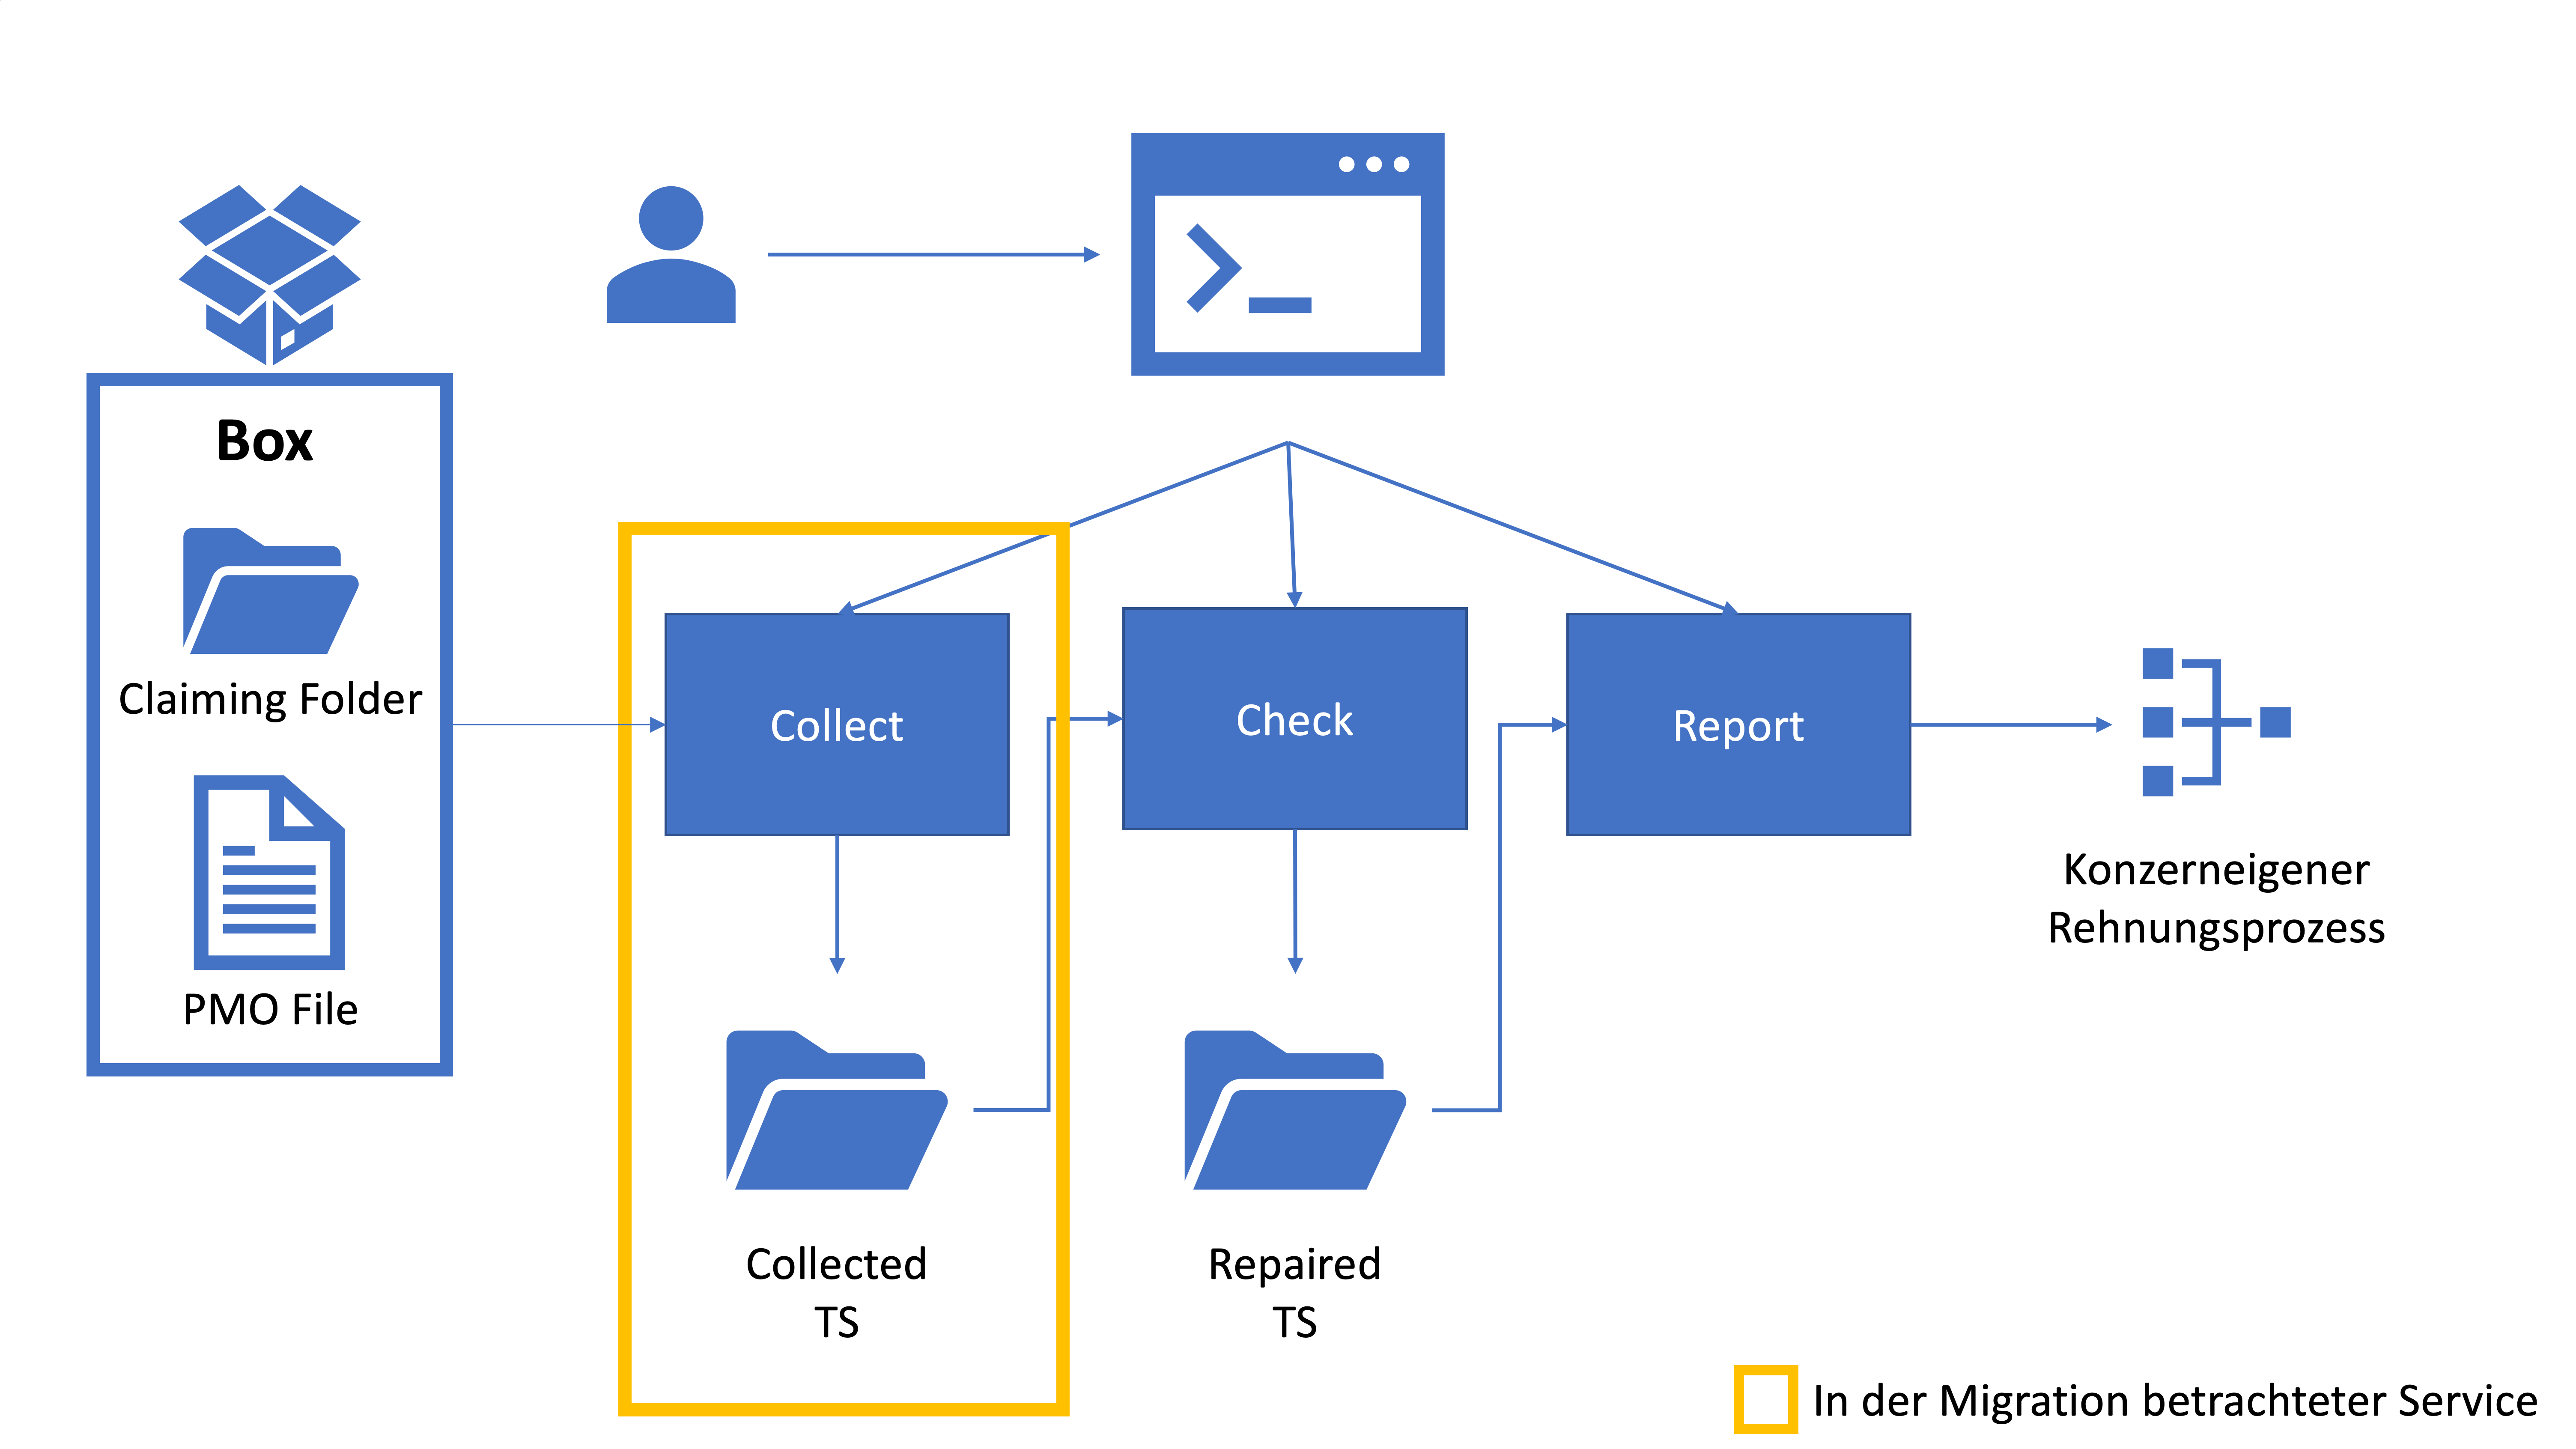
\includegraphics[width=0.65\textwidth]{pmo_python.png}
    \caption{Aufbau der ursprünglichen Anwendung (gelb umrandet der Teil, der prototypisch migriert wird)}
    \label{fig:pmo_python}
\end{figure}

Die bisher existierende Anwendung ist eine Python Anwendung, die grundsätzlich in dre Module aufgeteilt ist:
\begin{itemize}
\item \textbf{Timesheet Collector: }Einsammeln der Timesheets der in dem Projekt aktiven Mitarbeiter
\item \textbf{Timesheet Checker: }Überprüfen der Timesheets auf Korrektheit uns Vollständigkeit und gegebenenfalls Reparatur dieser
\item \textbf{Report Creator: }Erzeugung eines Reports und automatisierte Rechnungsstellung
\end{itemize}

Jeder dieser drei Services ist ein eigenes Python Modul. Diese greifen jeweils auf weitere Services wie einen Excel-Helper und Checking-Tools zurück.

Da es sich bei dieser Arbeit um eine Machbarkeitsstudie mit Erstellung eines Prototypen handelt, wird im ersten Schritt nur die Migration des Collect Service untersucht, bevor die anderen, komplexeren Services migriert werden. Dies ist in Abbildung \ref{fig:pmo_python} entsprechend durch den gelben Rahmen gekennzeichnet. Der Collect Service benötigt eine Verbindung zu dem Box-Verzeichnis und einen Ablageort für die \glqq{eingesammelten}\grqq{} Timesheets.

\subsection{Anforderungen an die Cloud Migration}
Wird eine Anwendung in die Cloud migriert werden unter anderem folgende Vorteile erwartet \cite[Vgl. auch im Folgenden][03:23-05:36min]{AWS2019}:
\begin{itemize}
\item Kostensenkung
\item Steigerung der Produktivität
\item Agilität in der Entwicklung
\end{itemize}

Darüber hinaus muss vor der Migration untersucht und festgelegt werden, welche der in Kapitel \ref{sec:migrationsansaetze} herausgearbeiteten Migrationsstrategien verfolgt werden soll \cite[Vgl.][10:38-13:23min]{AWS2019}. Jede dieser Strategien bietet ihre Vor- und Nachteile, weshalb diese Entscheidung individuell von der Anwendungsarchitektur und der Art der Benutzung abhängig ist. \pagebreak

Grundlegend kann der Migrationsprozess  in vier Schritte zusammengefasst werden \cite[Vgl. auch im Folgenden][S. 34f]{Maenhaut2016}:
\begin{enumerate}
\item \textbf{Auswahl der Komponenten:} Die Auswahl der zu migrierenden Komponenten sollte als erster Schritt vorgenommen werden. Wird die ganze Anwendung migriert ist dieser entsprechend einfach. Zu beachten ist hier vorallem die Kommunikation zwischen den Komponenten und damit verbundenen Sicherheitsanforderungen.
\item \textbf{Feststellen kompatibler Provider:} Verschiedene Provider bieten verschiedene Möglichkeiten und haben unterschiedliche limitierende Faktoren. Somit sollte ein Provider gefunden werden, der alle gewünschten Features abdecken kann.
\item \textbf{Einfluss auf das Client Netzwerk untersuchen:} Da die Kommunikation zwischen einzelnen Komponenten ins Internet verlagert wird, muss möglicher Weise die Bandbreite des Client Netzwerks angehoben werden.
\item \textbf{Skalierung der Anwendung:} Einer der Vorteile des Cloud Computing ist die Skalierbarkeit, also die Fähigkeit, bei großer Last weitere Instanzen einer Anwendung zu starten. Um diese Skalierbarkeit bereitstellen zu können müssen die Komponenten lokalisiert werden, die entsprechend angepasst werden müssten.
\end{enumerate}

Bei dem in dieser Arbeit untersuchten Prototypen werden alle Komponenten des Collect Service migriert, weshalb keine speziellen Komponenten ausgewählt werden müssen oder die Kommunikation zwischen diesen geprüft werden muss. Somit ist der erste Schritt recht einfach abzuschließen. Die Auswahl eines Passenden Providers wird im weiteren Verlauf dieser Arbeit beschrieben. Einen Einfluss auf das Client Netzwerk wird der Prototyp nicht haben, es sollte lediglich hinsichtlich der Auswahl des Cloud Providers darauf geachtet werden, dass die Netzwerkanbindung ausreicht um zum Beispiel das Projektmanagement-File zuverlässig herunterzuladen. Die Skalierbarkeit der Anwendung bleibt für den ersten Prototypen vorerst außerhalb der Zielsetzung, diese würde erst nach einer erfolgreichen Machbarkeitsstudie weiter betrachtet werden.

Darüber hinaus soll eine Anwendung in der Cloud je nach Bedarf auch von mehr Nutzern gleichzeitig nutzbar sein, weshalb auch über die Umsetzung von \textit{multi-tenancy} nachgedacht werden sollte \cite[Vgl.][S. 34ff]{Maenhaut2016}. Im Falle des in dieser Arbeit beschriebenen Prototypen ist das jedoch erst einmal nicht nötig.
\pagebreak
% Use-Case Analyse
\section{Use-Case Modellierung}
\label{sec:use-case-modellierung}

Nachfolgend wird die ursprüngliche Anwendung funktional Beschrieben, um daraus die Qualitätsanforderungen für die Migrierte Anwendung abzuleiten. Durch das Testen auf die Qualitätsanforderungen soll untersucht werden, ob sich eine Veränderung im Nutzungsverhalten bei der Migration in die Cloud ergibt.

\subsection{Funktionale Beschreibung der bisherigen Anwendung}
Die Funktionalität der bisherigen Anwendung besteht darin, den Prozess der Rechnungsstellung zu automatisieren und somit management Aufwände zu reduzieren. Dazu besteht die Anwendung hauptsächlich aus drei Services, dem \textit{Collect Service}, dem \textit{Check Service} und dem dem \textit{Report Service}. Ausgeführt wird die Anwendung bisher auf einem lokalen System und greift über das lokale Verzeichnis mithilfe einer \gls{Box}-Integration auf diese zu. Zur Ausführung der Anwendung wird eine Konfigurationsdatei benötigt, die alle notwendigen Pfade und Parameter enthält. In dem \gls{Box}-Verzeichnis liegen die \textit{\glspl{Timesheet}} der Mitarbeiter des Projektes und eine Projektmanagementdatei (PMO-File), die allgemeine Informationen zum Projekt und den Mitarbeitern enthält.

Aufgabe des \textit{Collect Service} ist es, aus dem PMO-File oder einer alternativen Mitarbeiterliste alle, aktuell in dem Projekt aktiven Mitarbeiter zu ermitteln und die \textit{\glspl{Timesheet}} dieser in ein \textit{Collect}-Verzeichnis zu kopieren. Der \textit{Check Service} gleicht die von den Mitarbeitern manuell ausgefüllten \textit{\glspl{Timesheet}} mit den Daten aus einem Zeiterfassungstool und ermittelt, ob die Daten korrekt sind oder gegebenenfalls korrigiert werden müssen. Abschließend werden im \textit{Report Service} aus den Daten die Rechnungen für den Kunden erstellt, indem die Informationen aus den \textit{\glspl{Timesheet}} detailliert auf die einzelnen Teilprojekten aufgeteilt und abgerechnet werden.

In dieser Arbeit soll untersucht werden, ob sich eine Veränderung im Nutzungsverhalten bei der Migration in die Cloud ergibt und ob die Business-Logik entsprechend angepasst werden muss. \pagebreak

\subsection{Wie könnte ein Cloud Setup Aussehen?}
Durch die Migration in die Cloud ergeben sich viele Möglichkeiten für die Anwendung. Unter anderem bringt die Cloud-Migration \textit{\gls{Multi-Tenancy}}, also eine Mehrbenutzerfähigkeit mit sich, damit die Anwendung von mehreren Nutzern gleichzeitig verwendet werden kann, ohne dass diese sich beeinflussen oder behindern.

Um die Anwendung allgemein in die Cloud zu migrieren, könnte diese so wie sie ist mit \textit{Lift-and-Shift} in eine virtuelle Maschine Kopiert werden und würde somit in der Cloud bereitgestellt. Dadurch könnte jedoch keine Aussage darüber getroffen werden, inwiefern die Anwendung oder ihre Architektur verändert werden muss, um die Vorteile einer Cloud-nativen Anwendung in der Cloud auszunutzen.

Aus diesem Grund soll die Anwendung zu einer Web-Anwendung weiterentwickelt werden. Dadurch verändert sich die Art und Weise, wie die Use-Cases Ausgeführt werden und wie die Anwendung benutzt wird. Diese Veränderungen werden am Beispiel der Migration des \textit{Collect Service} untersucht.

\subsection{Collect Service}
\textbf{Bisherige Verwendung:} Der für den Prototypen ausgewählte Use-Case ist das \glqq{Einsammeln}\grqq der \textit{\glspl{Timesheet}}. Aus einer Konfigurationsdatei hinaus soll festgelegt werden für welches Projekt und welchen Zeitraum diese von dem Projektverzeichnis in ein temporäres Verzeichnis kopiert werden sollen. 

\textbf{Möglichkeiten einer Web-Anwendung:} Durch die Migration in die Cloud und die Weiterentwicklung zu einer Web-Anwendung können die Funktionen der Anwendung zukünftig über einen API-Endpunkt bereitgestellt werden und die Ausführung dieser kann zum Beispiel nach einem Zeitplan oder einem Trigger, wie das Hochladen einer neuen Konfigurationsdatei erfolgen. Auf die hierzu notwendigen technischen Veränderungen wird später in der Arbeit eingegangen. \pagebreak

\textbf{Use-Case Definition:} Nachfolgend wird der Use-Case definiert, um im Anschluss an die Implementierung untersuchen zu können, ob dieser auch nach der Migration in die Cloud erfüllbar ist.

\begin{figure}[H]
    \centering
    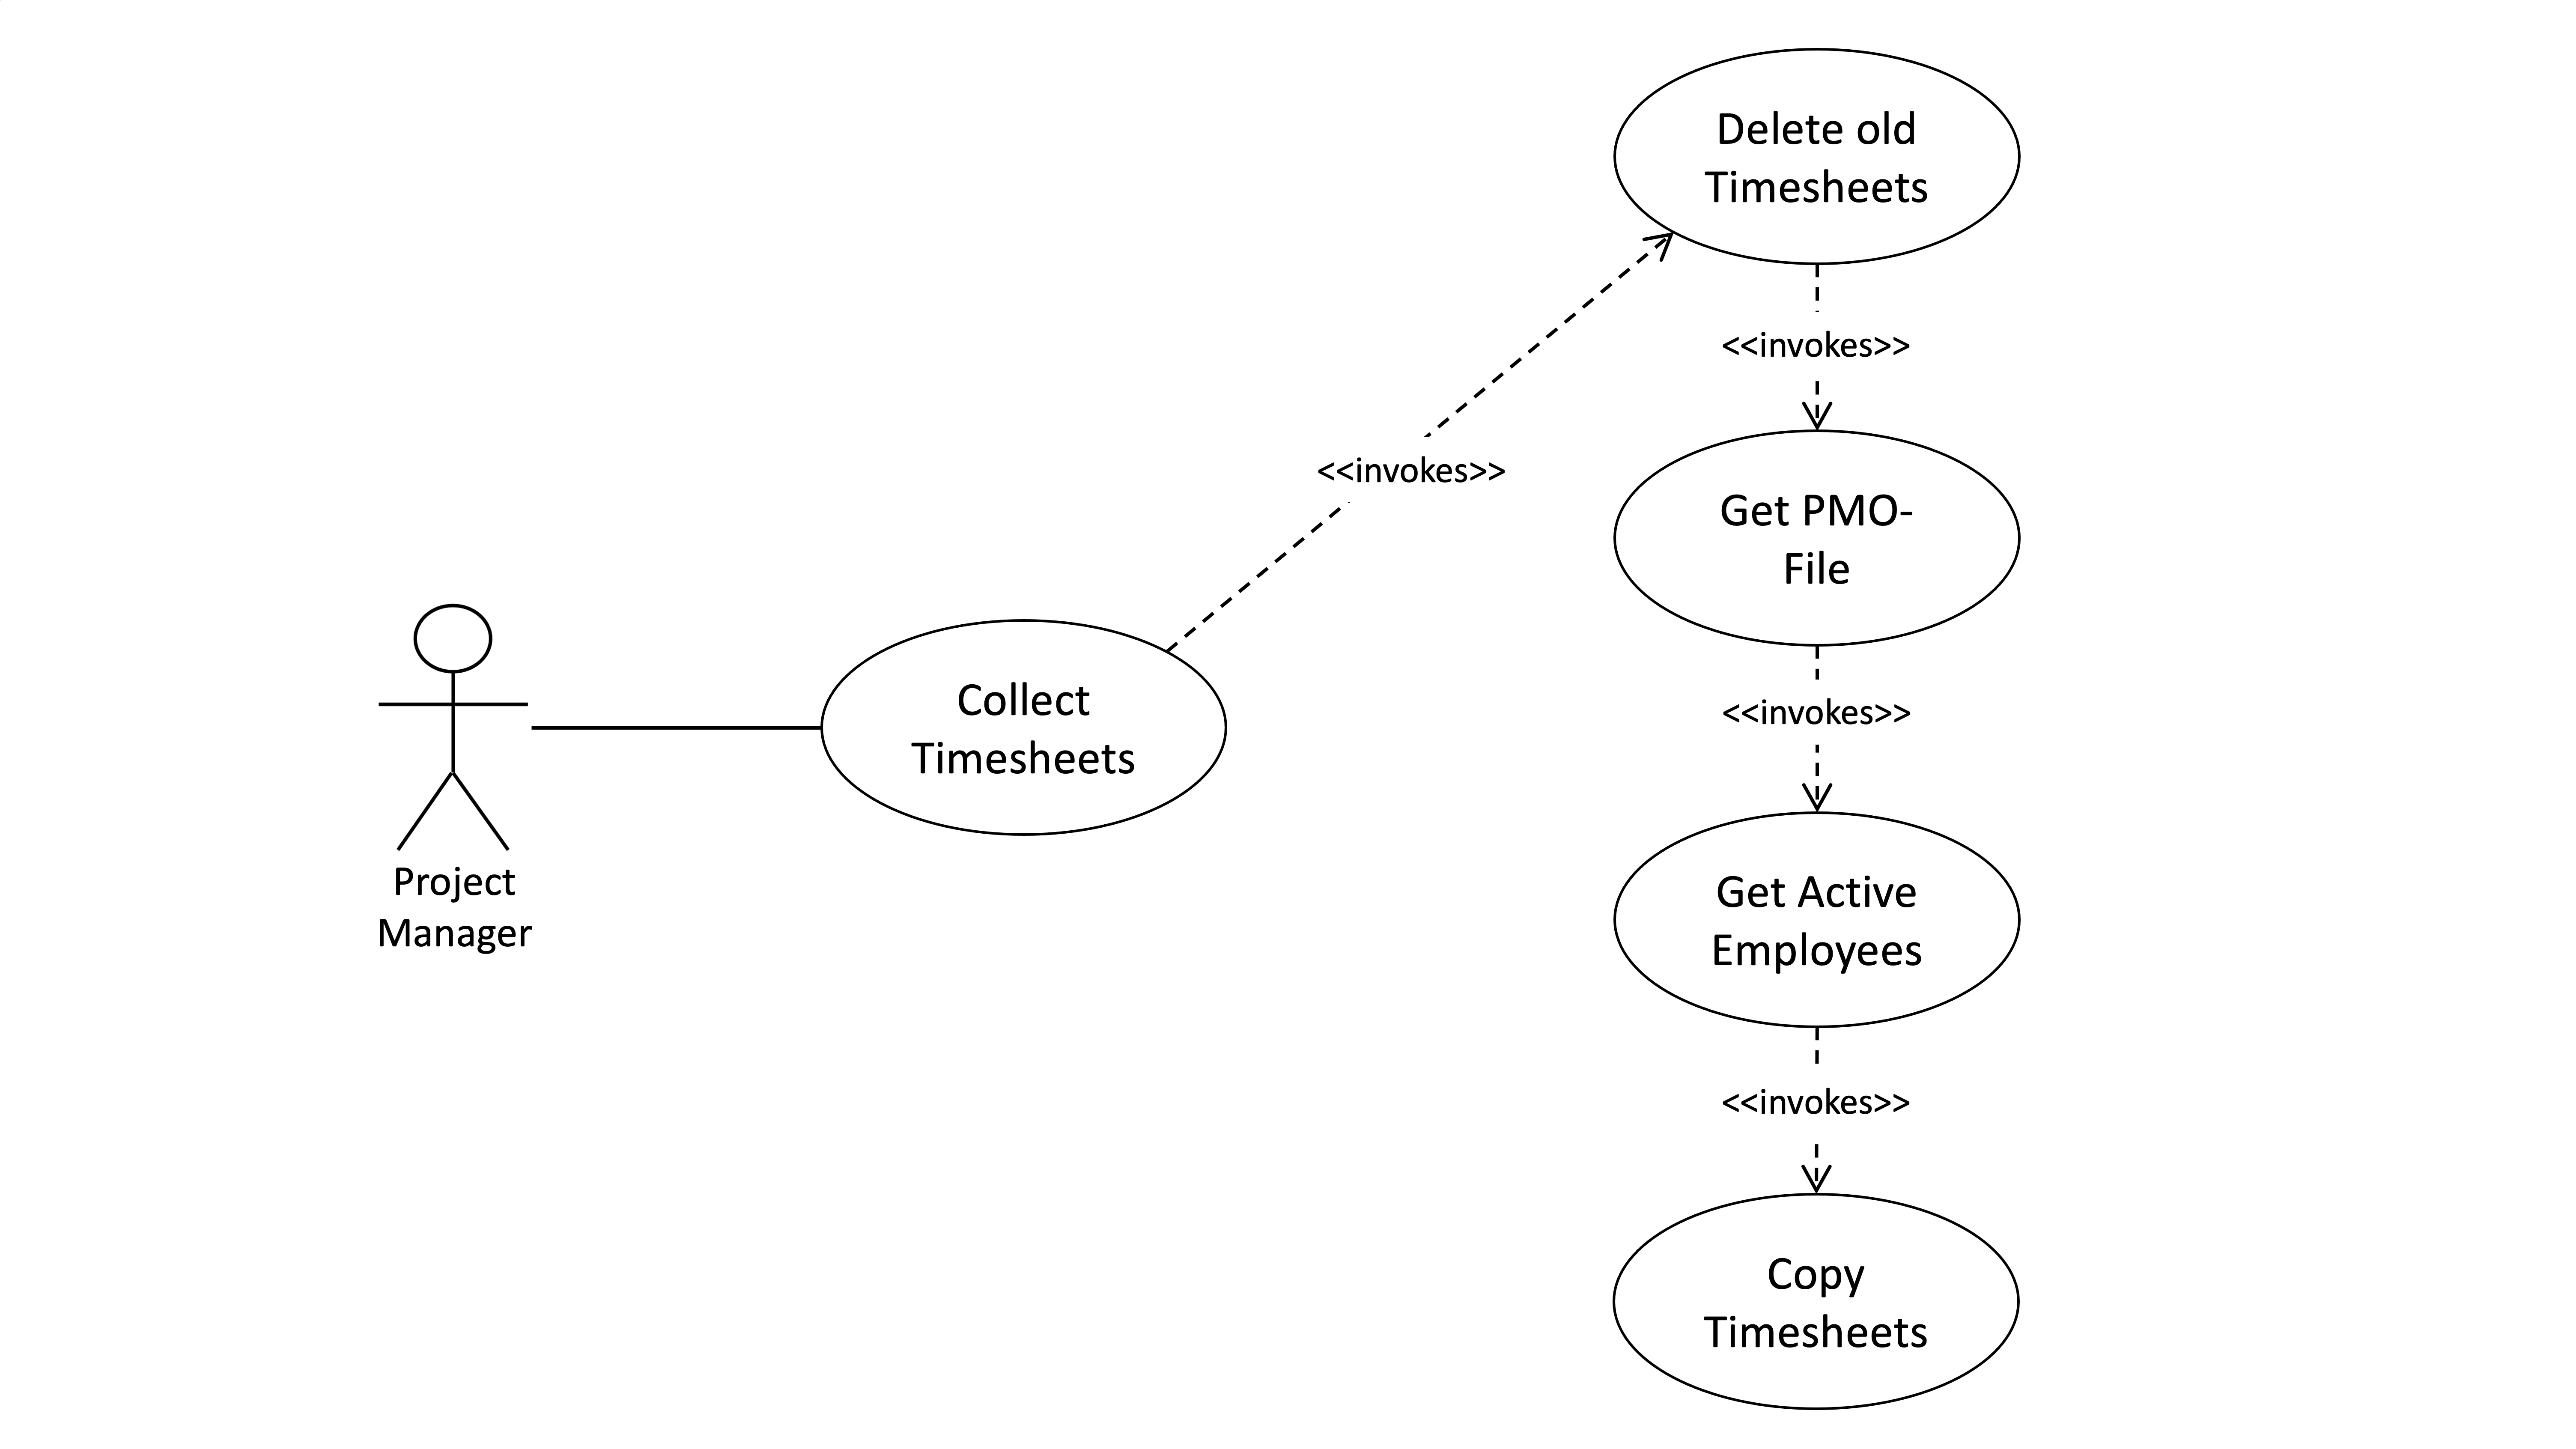
\includegraphics[width=\textwidth]{use-case-diagram.png}
    \caption{Use-Case Diagramm}
    \label{fig:use-case-diagram}
\end{figure}

Abbildung \ref{fig:use-case-diagram} stellt grafisch dar, welche Aufgaben der \textit{Collect Service} erfüllen muss und in welcher Reihenfolge diese ausgeführt werden. diese grundlegende Funktionsweise darf durch eine Cloud Migration nicht beeinträchtigt werden.

\begin{table}[H]
    \begin{tabular}[H]{|l|l|}
        \hline
        \multicolumn{2}{|l|}{\textbf{Anwendungsfall:} Einsammeln der \textit{\glspl{Timesheet}}} \\
        \hline
        \textbf{Kurzbeschreibung:} & \textit{\glspl{Timesheet}} aktiver Mitarbeiter in temporäres Verzeichnis kopieren \\
        \hline
        \multicolumn{2}{|l|}{\textbf{Normalverlauf}} \\
        \hline
        \multicolumn{2}{|l|}{1. Leeren des temporären Ordners} \\
        \multicolumn{2}{|l|}{2. PMO Datei finden und laden} \\
        \multicolumn{2}{|l|}{3. Aktive Mitarbeiter aus PMO Datei lesen} \\
        \multicolumn{2}{|l|}{4. \textit{\glspl{Timesheet}} der aktiven Mitarbeiter kopieren} \\
        \hline
        \multicolumn{2}{|l|}{\textbf{Alternativablauf}} \\
        \hline
        \multicolumn{2}{|l|}{Siehe Normalverlauf} \\
        \multicolumn{2}{|l|}{\textbf{Qualitätsanforderungen}} \\
        \hline
        \multicolumn{2}{|l|}{1. Für jeden aktiven Mitarbeiter soll ein \textit{\gls{Timesheet}}im temporären Ordner liegen} \\
        \multicolumn{2}{|l|}{2. Die \textit{\glspl{Timesheet}} sollen unverändert sein (Dateiname, Inhalt)} \\
        \multicolumn{2}{|l|}{3. Eigener Zielordner pro Monat zur Vermiedung von Vermischungen} \\
        \multicolumn{2}{|l|}{4. Die \textit{\gls{Timesheet}} Größe kann variieren -> keine Limitierungen} \\
        \multicolumn{2}{|l|}{5. Es darf keine Kompression mit Formatänderung eingesetz werden} \\
        \multicolumn{2}{|l|}{6. Ein Logfile soll Erfolg und Misserfolg von Kopiervorgängen enthalten} \\
        \multicolumn{2}{|l|}{7. Fehlersituationen auf einzelnen Dateien dürfen den Ablauf nicht unterbrechen} \\
        \multicolumn{2}{|l|}{8. Root-Verzeichnisse für Ziel und Quelle müssen konfigurierbar sein} \\
        \hline
    \end{tabular}
    \caption{Anwendungsfall: Einsammeln der \textit{\glspl{Timesheet}}}
    \label{tab:use-case-analyse-timesheets}
\end{table}

Anschließend an diesen Prozess würden die weiteren Services der Toolsuite folgen, die für den Umfang dieser Arbeit ausgelassen wurden.
% 2. Entwicklung einer Cloud Nativen Anwendung
\chapter{Entwicklung einer Cloud-nativen Architektur}
\label{chapter:cloud-architektur}

\section{Konzeptentwurf der Anwendungsarchitektur}
\label{sec:konzeptentwurf}
Bevor die Anwendung in die Cloud migriert werden kann, muss konzeptioniert werden, wie die Anwendungsarchitektur aussehen soll und wie diese funktionieren wird. Dazu wurde vorangehend in der Anforderungsanalyse herausgearbeitet, welche Merkmale eine Cloud-native Anwendung erfüllen sollte, welche Migrationsstrategie verfolgt werden kann und welche Voraussetzungen dafür geschaffen werden müssen.

\subsection{Existierender Code}
Ziel der Anwendung ist das Einsammeln der \textit{\glspl{Timesheet}}, in dem Projekt aktiver Mitarbeiter, aus einem \gls{Box} Verzeichnis, das Überprüfen dieser und die anschließende Rechnungs- und Report Erstellung. Die Prozesse werden jeweils manuell über eine Konsoleneingabe gestartet. Im \gls{Box}-Verzeichnis liegt ein Projektmanagement-File, welcher alle Mitarbeiter enthält, die jemals in dem Projekt gearbeitet haben und markiert, welche auch aktuell aktiv sind und dem Kunden in Rechnung gestellt werden können. Außerdem sind in dem Verzeichnis auch die Reports aus einem Zeiterfassungstool abgelegt. In Abbildung \ref{fig:pmo_python} wird der Aufbau der ursprünglichen Anwendung dargestellt.

\begin{figure}[H]
    \centering
    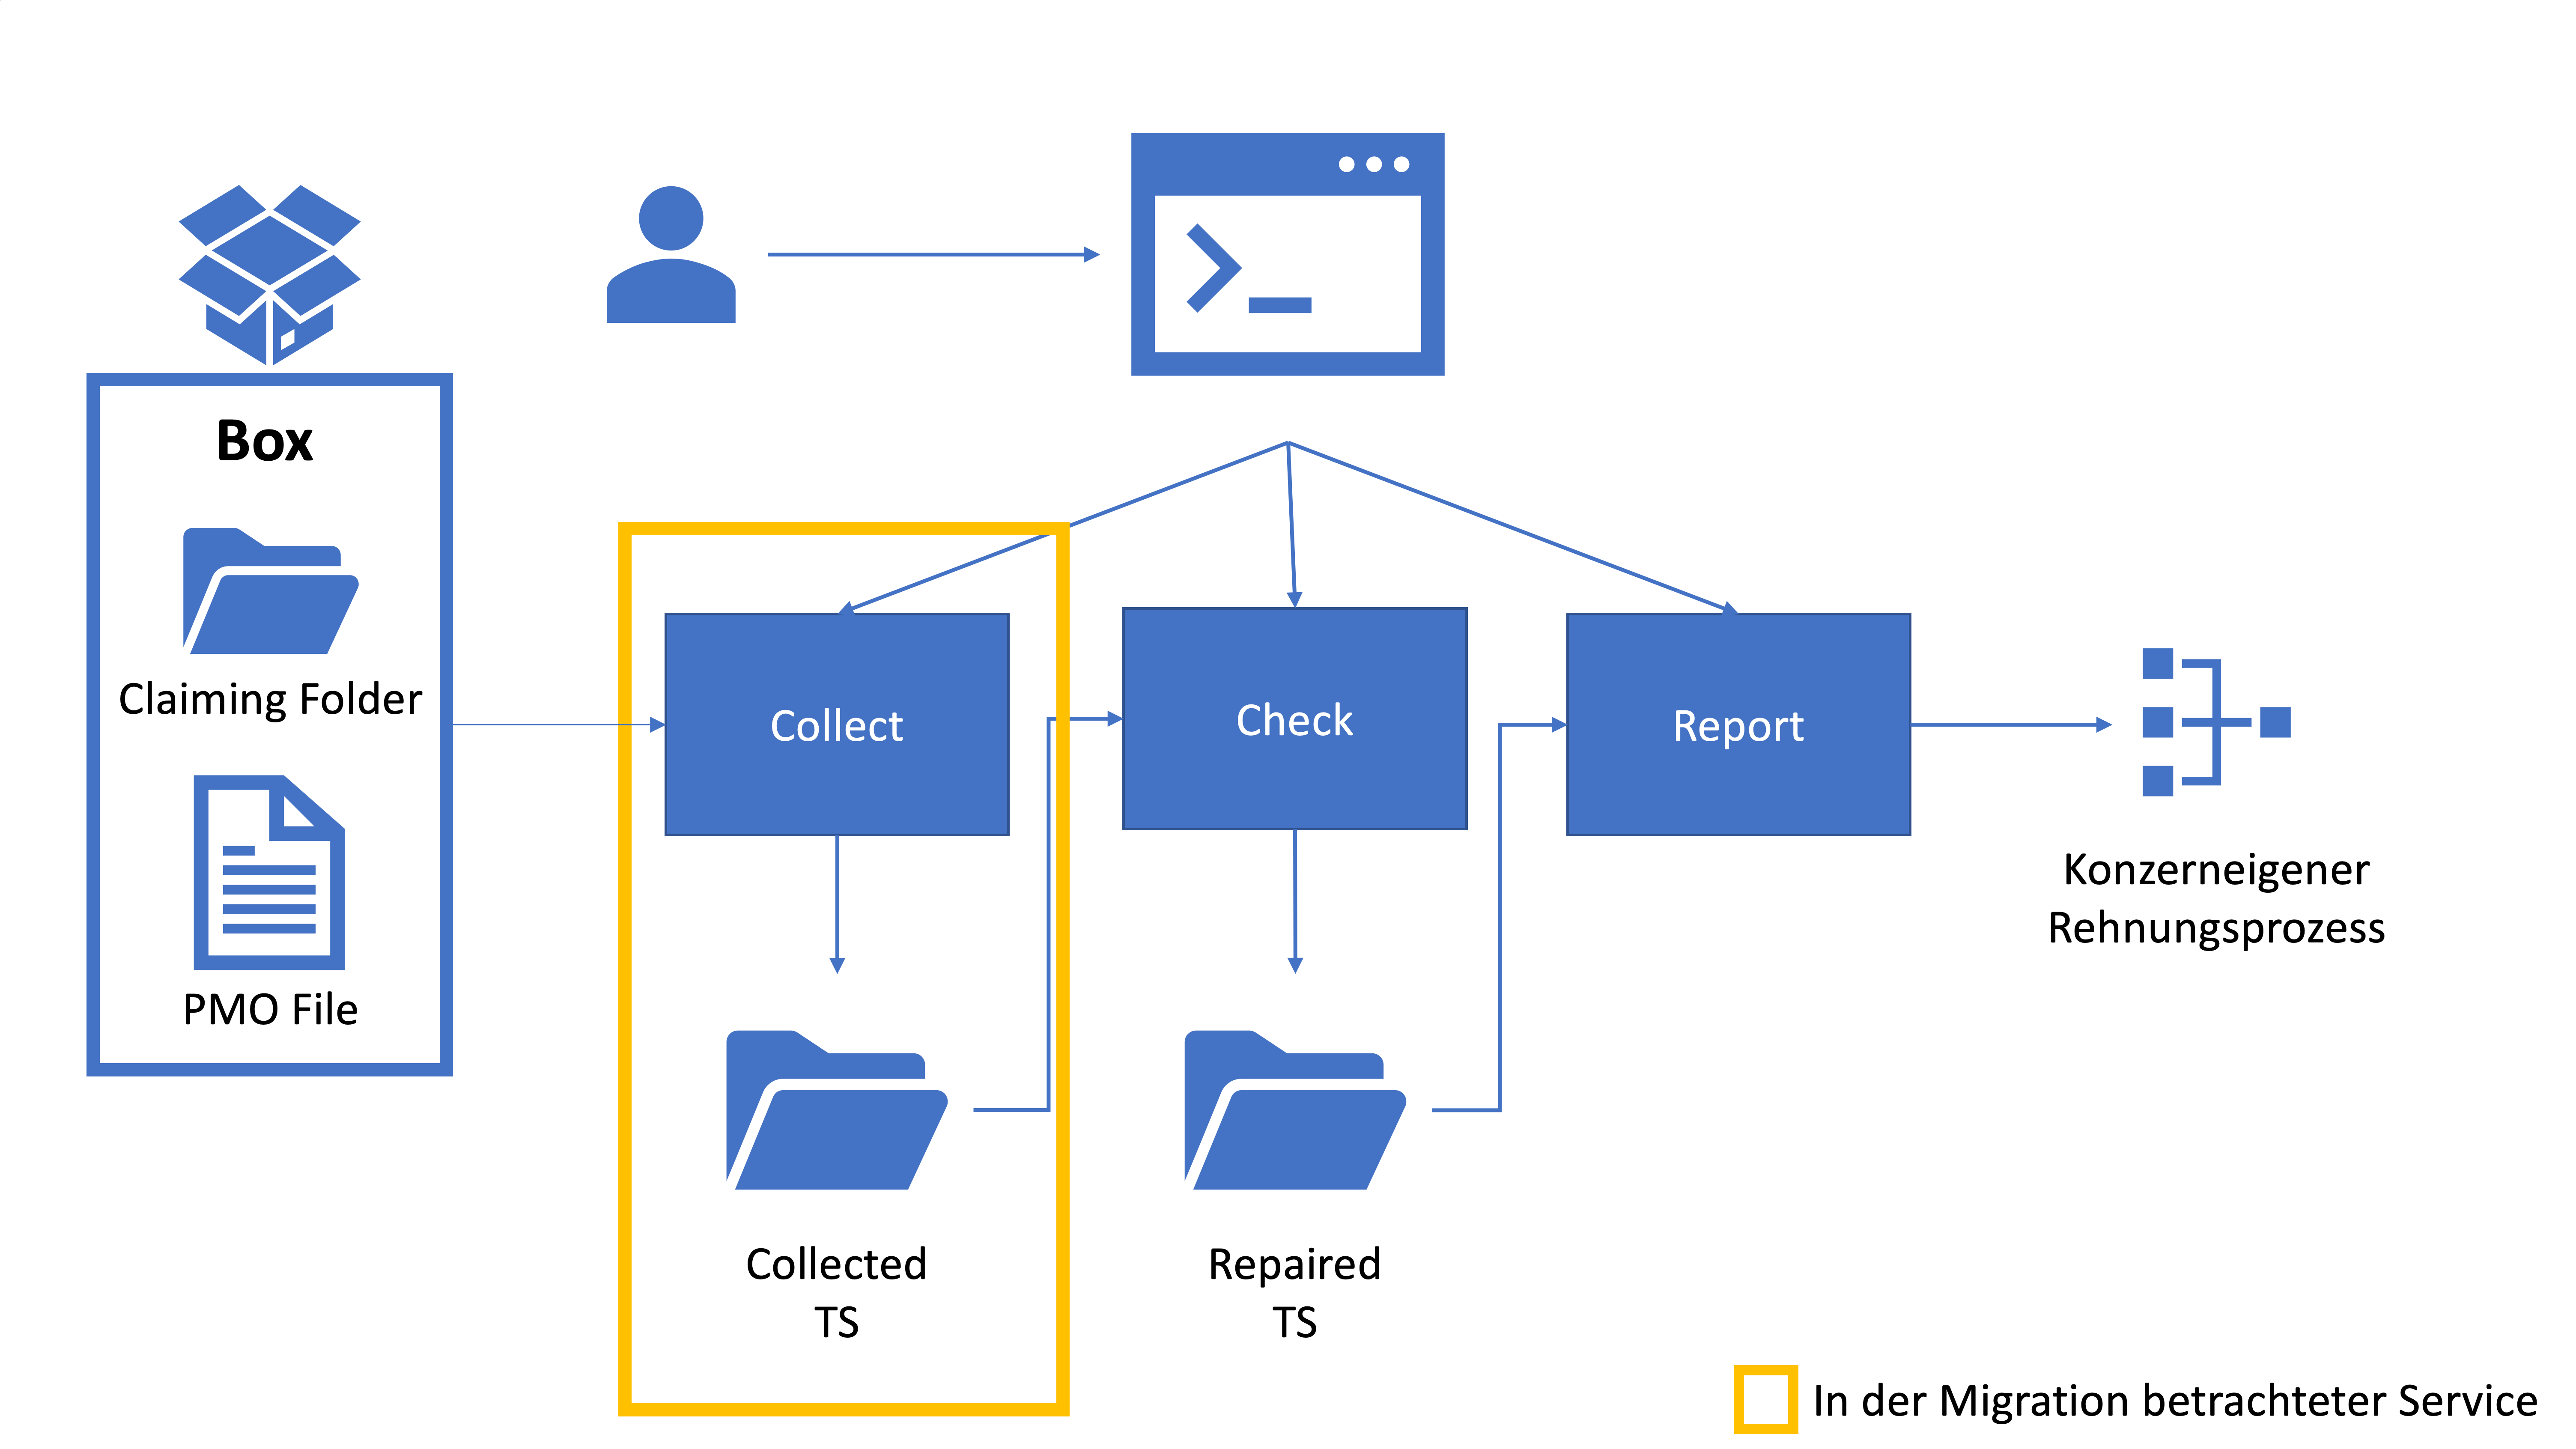
\includegraphics[width=0.65\textwidth]{pmo_python.png}
    \caption{Aufbau der ursprünglichen Anwendung (gelb umrandet der Teil, der prototypisch migriert wird)}
    \label{fig:pmo_python}
\end{figure}

Die bisher existierende Anwendung ist eine Python Anwendung, die grundsätzlich in drei Module aufgeteilt ist:
\begin{itemize}
\item \textbf{Timesheet Collector: }Einsammeln der \textit{\glspl{Timesheet}}, der in dem Projekt aktiven Mitarbeiter und Ablegen dieser in einem neuen Verzeichnis
\item \textbf{Timesheet Checker: }Überprüfen der \textit{\glspl{Timesheet}} auf Korrektheit und Vollständigkeit und gegebenenfalls Reparatur dieser (Fehlerkorrektur und Abgleich mit Daten aus Zeiterfassungstool zur Vermeidung von Unstimmigkeiten)
\item \textbf{Report Creator: }Erzeugung eines \textit{Reports}, Zusammenfassung der dokumentierten Stunden und Verteilung dieser auf die unterschiedlichen Beauftragungen, Erstellung von Nachweisdokumenten für die konzerneigene Rechnungsstellung
\end{itemize}

Jeder dieser drei Services ist ein eigenes Python Modul. Diese greifen jeweils auf weitere gemeinsame Services wie einen Excel-Helper und Checking-Tools zurück.

Da es sich bei dieser Arbeit um eine Machbarkeitsstudie mit Erstellung eines Prototypen handelt, wird im ersten Schritt nur die Migration des \textit{Collect Service} untersucht, bevor die anderen, komplexeren Services migriert werden. Dies ist in Abbildung \ref{fig:pmo_python} entsprechend durch den gelben Rahmen gekennzeichnet. Der \textit{Collect Service} benötigt eine Verbindung zu dem \gls{Box}-Verzeichnis und einen Ablageort für die ''eingesammelten'' \textit{\glspl{Timesheet}}.
\pagebreak

\subsection{Entwurf der neuen Architektur}
Kern der Anwendung soll trotz der Weiterentwicklung und anstehenden Änderungen die in Kapitel \ref{sec:use-case-modellierung} beschriebene Business-Logik bilden.

In der ursprünglichen Anwendung ist der Zugriff auf die \gls{Box} mithilfe eines zusätzlichen Desktop-Clients umgesetzt worden, welcher es ermöglicht, Verzeichnisse in \gls{Box} wie einen lokalen Dateipfad ansprechen zu können. Somit konnte der Box-Pfad in eine Konfigurationsdatei geschrieben und als Parameter an die Anwendung übergeben werden. Da in einem Container in der Cloud Umgebung kein Zugriff auf ein lokales Verzeichnis mit entsprechender \gls{Box}-Erweiterung in der selben Art und Weise hergestellt werden kann, muss hier in der neuen Anwendung entsprechend die \gls{Box}-\ac{API} eingebunden werden um den Zugriff auf die Verzeichnisse weiterhin zu ermöglichen. Insbesondere auch deshalb, weil die Mehrbenutzerfähigkeit gewährleistet werden soll, welche über ein lokales Verzeichnis nicht umsetzbar wäre. Hierfür stellt \gls{Box} selbst ein entsprechendes \ac{SDK} für diverse Sprachen bereit.

Außerdem enthalten die PMO-Tools ein Skript, welches den Umgang mit Excel Spreadsheets ermöglicht. Dazu gehört zum einen das Ermitteln aktiver Mitarbeiter und zum anderen das Auslesen der \textit{\glspl{Timesheet}}, was jedoch für den untersuchten Service vorerst keine Verwendung findet. Einen vergleichbaren Service muss auch die neue Anwendung zum Lesen des PMO-Files enthalten. Für andere Programmiersprachen, wie zum Beispiel Java kann man in diesem Fall auf \textit{Libraries} wie die \gls{Apache POI} Programmbibliothek zurückgreifen, welche das Lesen und Schreiben von Microsoft Office Dateien ermöglicht.

Den ''Hauptservice'' der Anwendung soll der \textit{\gls{Timesheet}}-Service bilden. Dieser soll alle Funktionen bereitstellen, die unter Verwendung der anderen Services die letztendlich gewünschte Funktionalität des Einsammeln der \textit{\glspl{Timesheet}} bieten. Darüber hinaus soll dieser für eine spätere Anwendungsversion auch die anderen Funktionalitäten aus der ursprünglichen Anwendung bereitstellen. In der ursprünglichen Anwendung wurden die Services durch eine Konsoleneingabe im Terminal gestartet. Dies ist so bei der Cloud Anwendung nicht mehr ohne weiteres möglich, weshalb die Anwendung zukünftig über einen \ac{API}-Endpunkt bereitgestellt wird. \pagebreak

Abbildung \ref{fig:Architektur} zeigt einen groben  Entwurf der Anwendung und wie die Services miteinander kommunizieren sollen. Der \textit{\gls{Timesheet}} Service soll zu einem späteren Zeitpunkt alle Funktionen aus der Ursprünglichen Anwendung bündeln, für den Prototypen wird sich jedoch, wie bereits in der Anforderungsanalyse erwähnt, auf den \textit{Collect Service} beschränkt.

\begin{figure}[H]
    \centering
    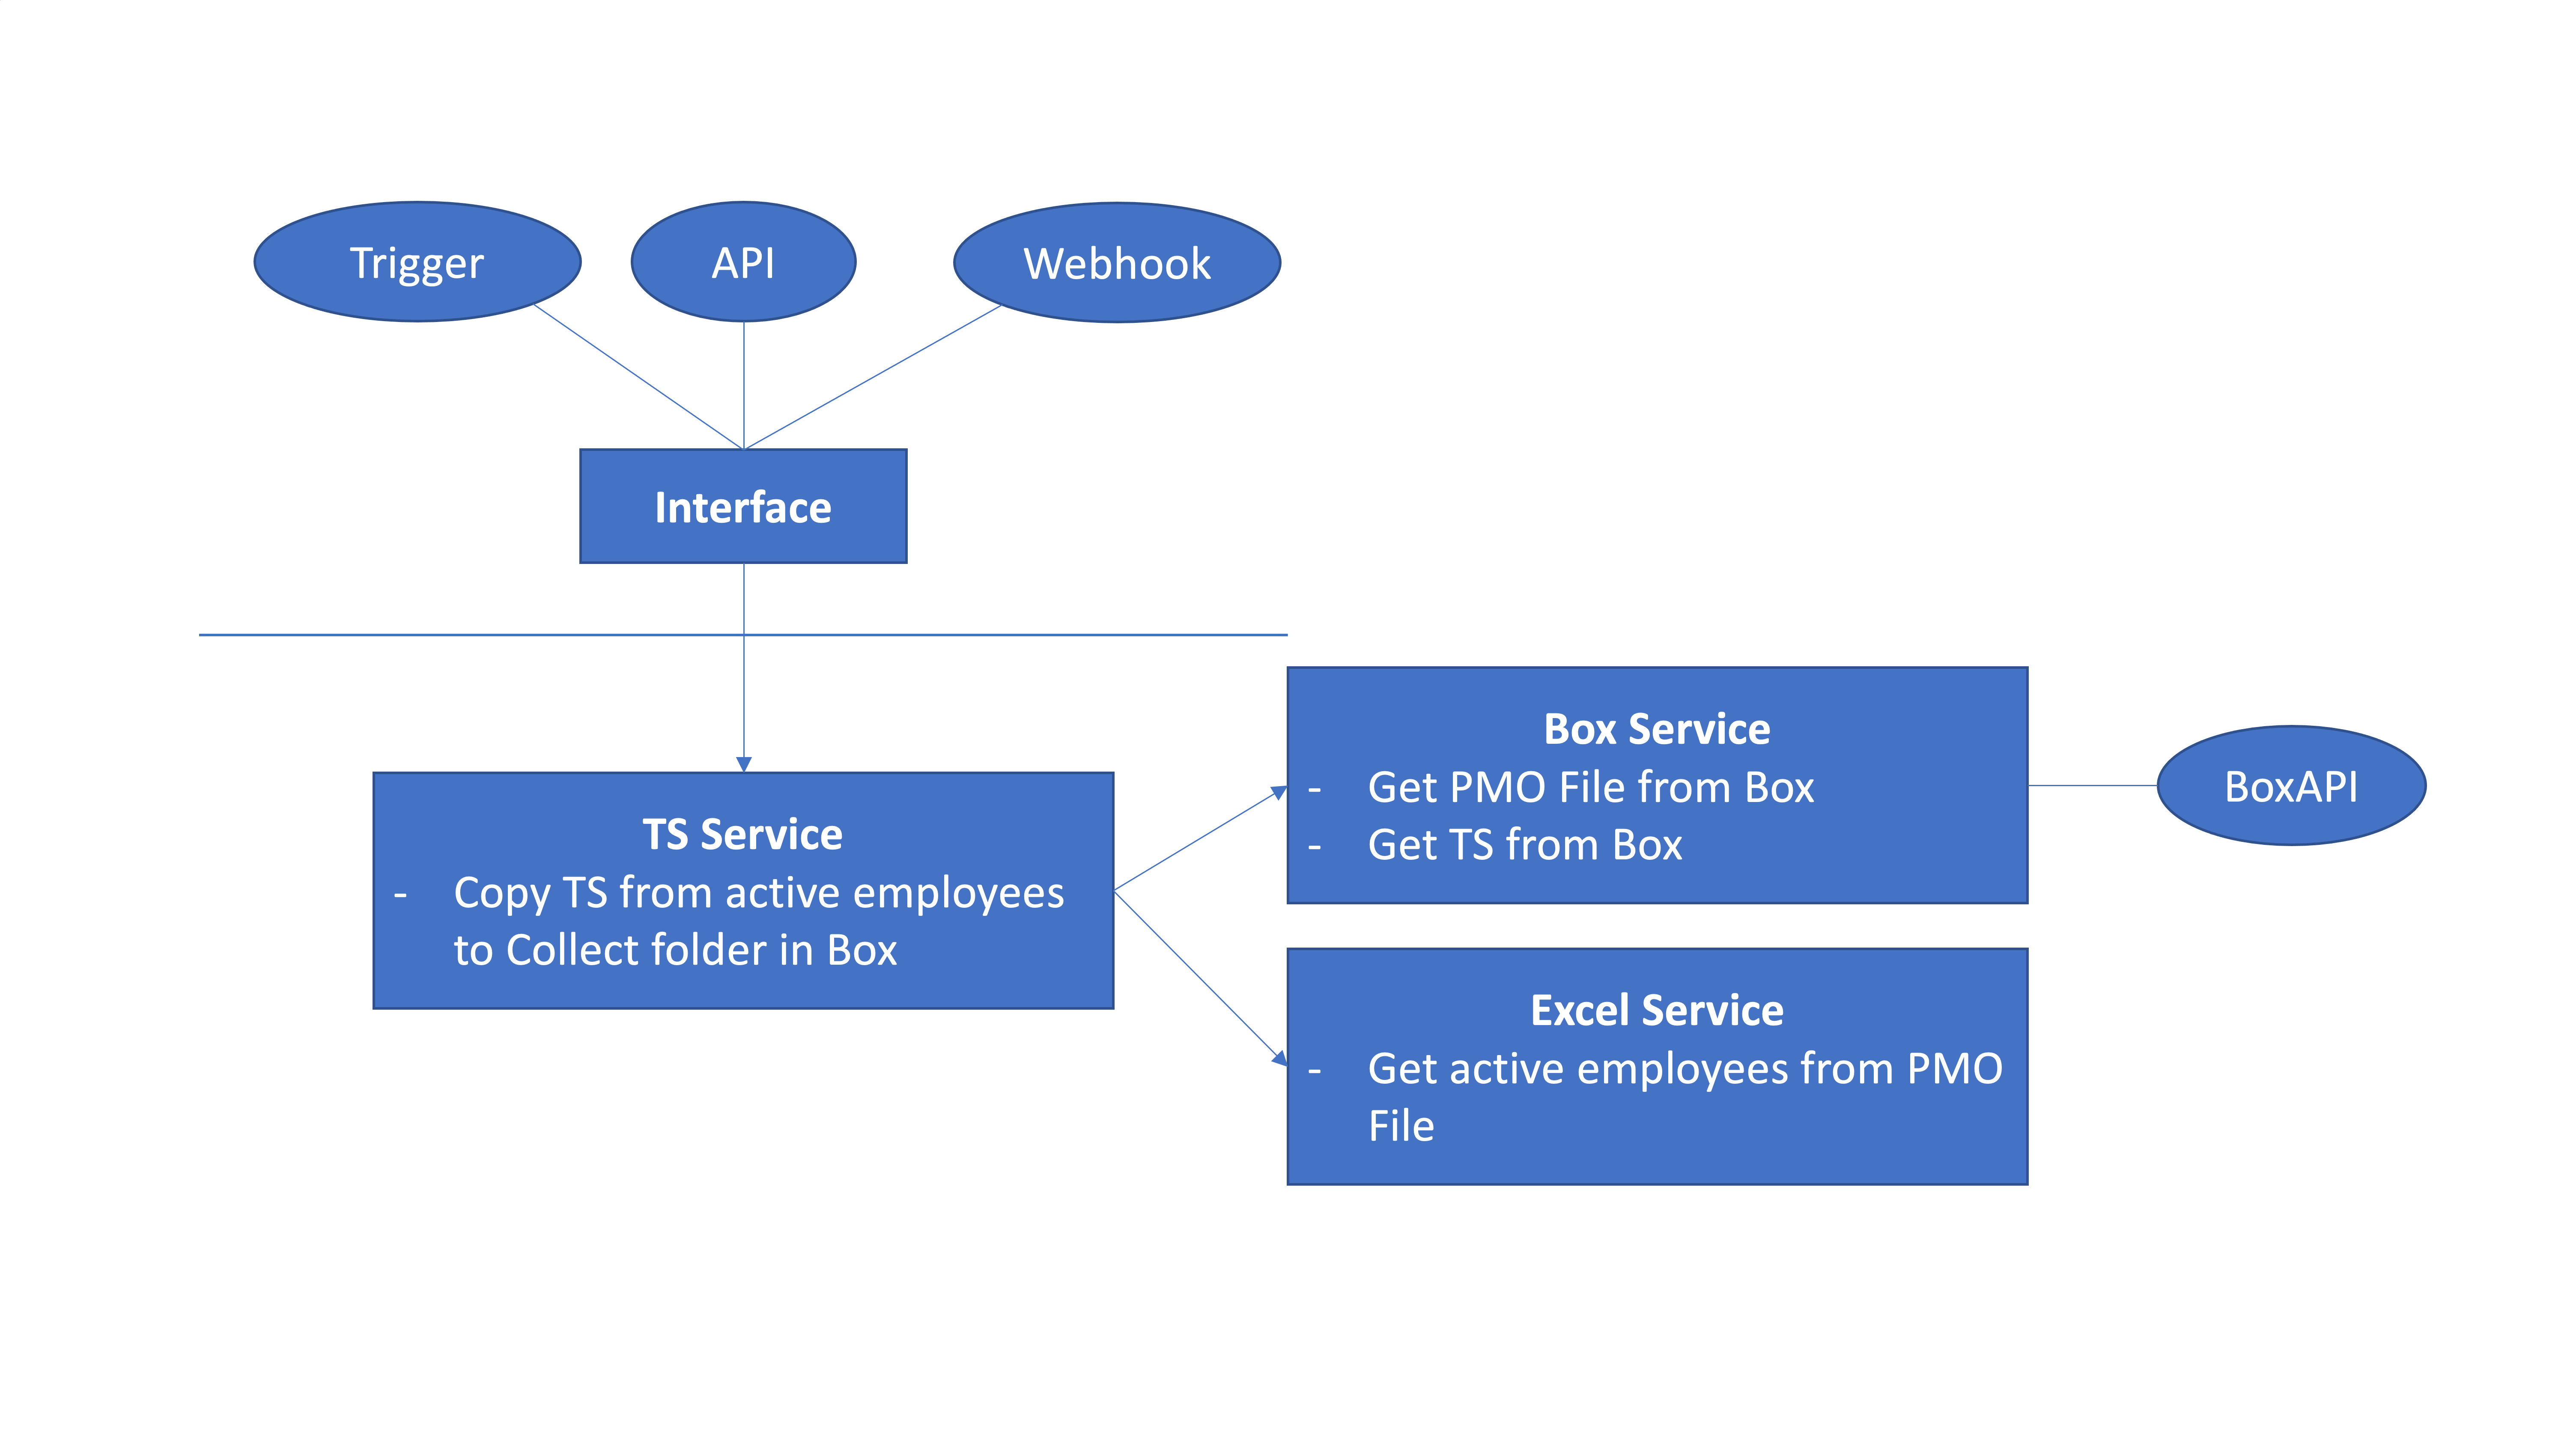
\includegraphics[width=\textwidth]{architektur.png}
    \caption{Architekturentwurf der neuen Anwendung}
    \label{fig:Architektur}
\end{figure}

In dem Prototypen wird die Anwendung über eine \ac{API} bereitgestellt werden. \textit{Trigger}\footnote{dt. Auslöser, z. B. durch Hochladen einer neuen Konfigurationsdatei} und \textit{Webhook}\footnote{Eigenwort, z. B. durch \gls{Box}-API bereitgestellte Verknüpfung zur Überwachung eines Ordners, Funktion ähnlich zu Trigger}, wie in der Abbildung dargestellt sollen visualisieren, dass auch alternative Interfaces eingesetzt werden können, ohne die Funktionalität der Anwendung zu beeinflussen. Neben der Erfüllung dieser funktionalen Anforderungen sollen auch die nicht-funktionalen Aspekte betrachtet werden. Dazu gehören die in Kapitel \ref{sec:anforderungsanalyse} erarbeiteten Anforderungen an eine Cloud-native Anwendung, unter anderem die Skalierbarkeit und Fehlertoleranz. Diese sollen über die in Kapitel \ref{sec:cloud-infra} konzipierte Cloud Infrastruktur in \ac{AWS} ermöglicht werden. \pagebreak

\subsection{Programmiersprache und Framework}
% Dependecy Injektion sehr gut (Austauschbarkeit der Implementierung)
% Spring MVC für REST-Anwendung in Springboot enthalten (Teil des Spring-Frameworks)
Neben der Konzeptionierung einer Anwendungsarchitektur braucht es zur Entwicklung auch eine Programmiersprache und gegebenenfalls ein Framework, um die Anwendung optimal in der Cloud beziehungsweise als Web-Anwendung nutzen zu können. 

Im Falle der PMO-Tools wurde ursprünglich Python verwendet, jedoch erschien im Zuge des Refactoring ein Wechsel zu Java und dem \gls{Spring} Framework sinnvoll, da hier mit \gls{Spring Boot} die Cloud-native Entwicklung erleichtert wird. Darüber hinaus gilt \gls{Spring Boot} als populärer Standard für den Einsatz von Microservices und die Bereitstellung einer \ac{REST}-\ac{API} ist mit \gls{Spring Boot} einfacher umzusetzen, da mit \textit{Spring MVC} bereits ein Web-Framework in \gls{Spring} enthalten ist, zur Bereitstellung von \ac{REST}-Endpunkten.

\subsection{Auswahl eines Cloud Providers}
Ein für die Cloud Migration unerlässlicher Schritt ist die Auswahl eines zu den Anforderungen passenden Cloud Providers. In diesem Fall wurde \ac{AWS} als einer der größten Provider \cite[Vgl.][S. 6]{Sustar2022} gewählt, da hier mit \ac{ECS} und \gls{Fargate} gute Möglichkeiten zum serverless Deployment von Containern zur Verfügung stehen um somit die Vorteile der Cloud optimal nutzen zu können. Darüber hinaus unterstützt \ac{AWS} viele offene Standards und Open-Source Tools, wie zum Beispiel \ac{IaC} mit Terraform.

Alternativ wurden auch die Services der IBM-Cloud in Betracht gezogen, da hier mit \textit{Cloud Functions} oder \textit{CodeEngine} ebenfalls Plattformen zum Deployment von Containern existieren, die jedoch zum einen schwieriger aufzusetzen schienen und zum anderen bezüglich der Möglichkeiten nicht mit \ac{ECS} vergleichbar sind. Ebenfalls hätte Azure, die Cloud Plattform von Microsoft infrage kommen können, da jedoch \ac{AWS} auch im Projektumfeld eingesetzt wird, wurde diese Alternative bevorzugt. \pagebreak
\section{Cloud Architektur}
In diesem Kapitel wird auf die verwendete Infrastruktur Architektur in \ac{AWS} eingegangen. Die nachfolgende Abbildung gibt einen Überblick wie die einzelnen Komponenten miteinander kommunizieren und voneinander abhängen. Drüber hinaus werden einige Gründe für die Auswahl der Services aufgezeigt.

\begin{figure}[H]
    \centering
    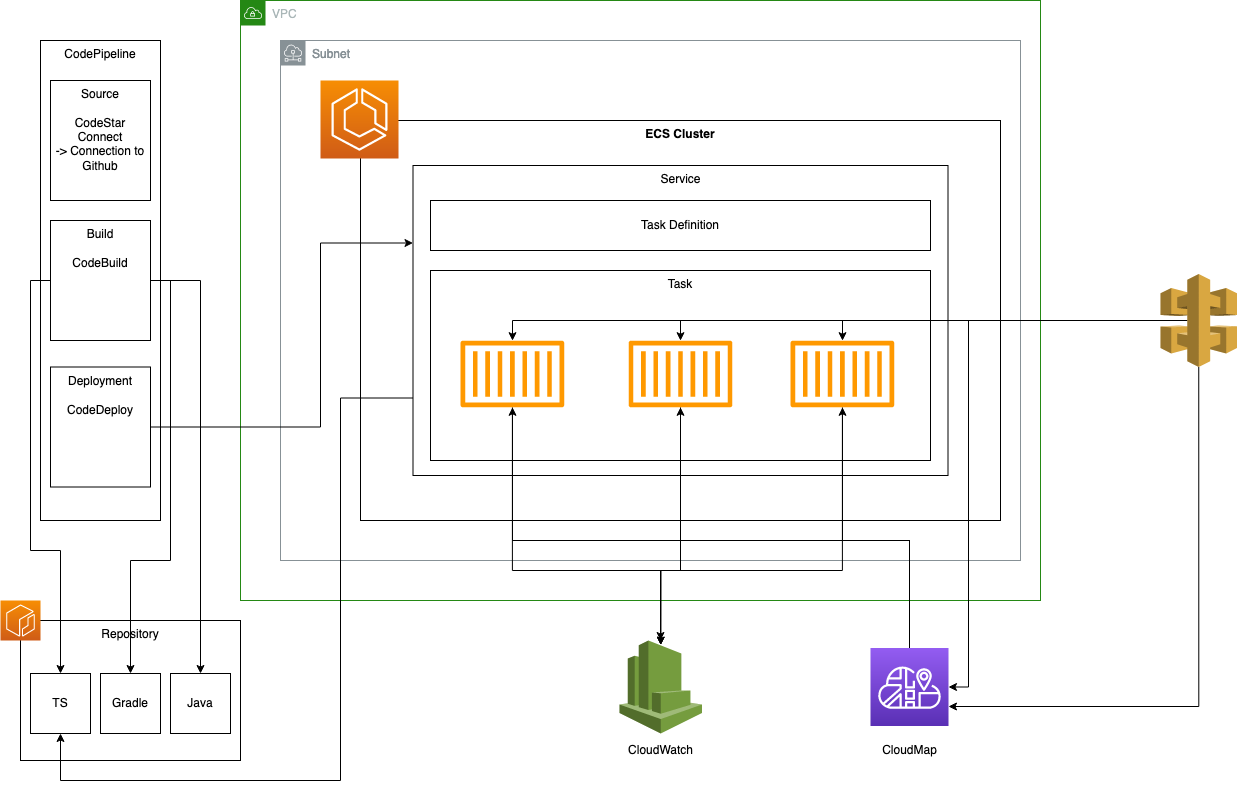
\includegraphics[width=\textwidth]{aws_architecture.png}
    \caption{Architekturentwurf für die AWS-Services}
    \label{fig:CloudArchitektur}
\end{figure}

Ziel ist es, die Anwendung auf Containern zu deployen. Dazu wird \ac{ECS} mit einem \gls{Fargate}-Worker eingesetzt zur Bereitstellung eines Clusters mit serverless Containern. Innerhalb des Clusters ist in einer \textit{Taskdefinition} festgelegt, wie viele Container gestartet werden sollen und die \textit{Task} selbst, in welcher die Container bereitgestellt werden.

Das \ac{ECS} Cluster selbst befindet sich innerhalb eines von einer \ac{VPC} bereitgestellten Subnetz. Erreichbar sind die einzelnen Container über ein \textit{\ac{API} Gateway}, welches auf die IP-Adressen innerhalb des Subnetzes verweist. Die Adressen der Container werden in \textit{CloudMap} gespeichert und der Betrieb dieser mit \textit{CloudWatch} überwacht.

Neben dem \ac{ECS} Cluster wird als weiterer Service \textit{\gls{CodePipeline}} eingesetzt. Dieser Kombiniert die Services \textit{CodeStar}, \textit{CodeBuild} und \textit{CodeDeploy}. \textit{CodeStar} stellt hierbei eine Verbindung zu \gls{GitHub} her, wo der Anwendungscode abgelegt ist. \textit{CodeBuild} erzeugt ein Abbild der Anwendung in einem Container und legt diesen in \ac{ECR} ab. \textit{CodeDeploy} deployt die aktuellste Version der Anwendung aus \ac{ECR} in das Cluster.
% 3. Implementierung des Prototypen
\chapter{Implementierung des Prototypen}

Nachfolgend wird die Implementierung des Prototypen beschrieben, bevor die notwendigen Schritte zur Cloud Migration der in dieser Arbeit untersuchten Anwendung zusammenfassend wiedergegeben werden, um einen Überblick über den Migrationsprozess zu geben.

\section{Lokale Implementierung der Anwendungsarchitektur}
% 1. Prototyp mit Mocks um Module einzeln und unabhängig voneinander oder von Daten zu testen
% 2. Schrittweise ersetzen der Mocks durch Verknüpfung der Module und Anbindung der Box-API
% 3. Bereitstellung der Anwendung über API

Wie bereits im vorangehenden Kapitel erarbeitet, soll die untersuchte Anwendung für die Cloud Migration in eine \gls{Spring Boot}-Anwendung umgewandelt werden. Die neue Anwendung wird im ersten Entwicklungsschritt auf einem lokalen System implementiert und getestet, bevor diese in die Cloud migriert wird.

Schritt für Schritt werden hierzu die Business-Logik der ursprünglichen Anwendung reproduziert und die \gls{Box}-\ac{API} eingebunden. Dazu werden die einzelnen Services nacheinander prototypisch entwickelt und mithilfe von Mock-Daten unabhängig voneinander getestet. Diese Mocks werden dann Schrittweise durch die Verknüpfung der einzelnen Services und das Einbinden der \gls{Box}-\ac{API} ersetzt. Schwierigkeiten haben sich dadurch vorallem durch Unvollständigkeiten in der \ac{API}-Dokumentation von \gls{Box}. Um die Anwendung ansprechen zu können wurden außerdem Endpoints definiert und über eine \ac{API} bereitgestellt.

Anschließend wird die Anwendung containerisiert. Dazu wird ein \textit{Dockerfile} definiert, in welchem die Schritte beschrieben sind, wie ein Docker-Image der Anwendung erstellt werden kann.

Um die Funktionen der neuen \gls{Spring Boot} Anwendung zu testen werden Testdatensätze nach dem Vorbild der realen Daten erstellt und in ein \gls{Box}-Verzeichnis gelegt. Über die von der Anwendung bereitgestellte \ac{API} können nun die Funktionen der Anwendung getestet werden. \pagebreak

\section{Bereitstellung in der Cloud}
% Lokal im Container laufende Anwendung
% Zuvor definierte Infrastruktur mithilfe von Terraform aufgesetzt (-> reproduzierbar)
% - Aufsetzen einer CodePipeline zur automatisierten Bereitstellung
% Schreiben der TaskDefinition um Container als workload in ECS auszuführen
% Initiale Ausführung von CodePipeline
% -> Build Anwendung
% -> Build + Push Image
% -> Deployment ECS
% => Anpassung von Security Konfiguration notwendig
% Wieder die gleichen Tests wie lokal, diesmal gegen API Gateway API

Nachdem die Anwendung lokal bereits in einem Container bereitgestellt wird, kann diese nun in die Cloud migriert werden.

Die zuvor in Kapitel \ref{chapter:cloud-architektur} definierte Cloud-Infrastruktur wird in einem \gls{Terraform}-Skript aufgesetzt. Damit ist die Cloud-Umgebung jederzeit reproduzierbar. Hierin wird eine CodePipeline aufgesetzt um eine automatisierten Bereitstellung der Anwendung zu ermöglichen.

Um die Container als Workload in ECS auszuführen, wird außerdem eine \textit{TaskDefinition} über \gls{Terraform} erstellt. Diese beschreibt unter anderem, welches Anwendungsimage in einem Container deployed wird, wie viel Arbeitsspeicher und Prozessorleistung zur Verfügung gestellt werden und wie zum Beispiel mit dem Abstürzen eines Containers umgegangen werden soll \cite[Vgl.][]{AWSECS}.

Mit dem Aufsetzen der Cloud-Umgebung kann nun die Anwendung initial in der Cloud deployed werden. \textit{CodeStar} lädt den Anwendungscode aus dem \gls{Repository}, welcher dann von \textit{CodeBuild} als \textit{Image} gebaut und in der \ac{ECR} abgelegt wird. Dieses \textit{Image} der Anwendung kann dann in \ac{ECS} deployed werden.

Bei der Initialisierung der Anwendung ist aufgefallen, dass die Standard Sicherheitskonfiguration des Subnets der \ac{VPC} nicht den Anforderungen entspricht und Netzwerkverbindungen blockiert, die zur Ausführung der Anwendung notwendig sind. Diese Konfiguration muss entsprechend angepasst werden, damit die Services untereinander kommunizieren können und zum Beispiel die \gls{Box}-\ac{API} erreichbar ist. Zusätzlich sind noch Schwierigkeiten im Routing aufgetreten, da neben der eigentlichen \ac{API} zusätzlich noch ein \ac{API}-Gateway eingesetzt wurde.

Nachdem diese Probleme gelöst wurden, kann die migrierte Anwendung nun mit den gleichen Testdaten, wie die lokale Anwendung getestet werden.

% Zuerst wurde untersucht, welche Migrationsstrategie für die vorliegende Anwendung in Frage kommen könnte. Im vorliegenden Beispiel ist die Entscheidung auf ein Refactoring gefallen, um die Vorteile der Cloud mit einer Spring Boot Anwendung nutzen zu können. Ein Rehosting der existierenden Python Anwendung wäre dazu nicht ausreichend gewesen, da der Service zwar in einem Container laufen würde, jedoch ohne die Vorteile der Cloud nutzen zu können, da diese dann zwar über das Internet erreichbar wäre, aber sich die Art der Ausführung dieser im Vergleich zu einer lokalen Anwendung nur geringfügig ändert.

% Um testen zu können, ob die Migration in diesem Fall überhaupt die gewünschten Vorteile mit sich bringt, wurde außerdem entschieden, für die erste testweise Umsetzung nur einen der vier Services zu migrieren. Für diesen Service wurde anschließend konzeptioniert, wie die Funktionen der Anwendung nun in Spring umgesetzt werden können, um der ursprünglichen Funktionalität zu entsprechen. Darüber hinaus musste dann für die Anwendung auch ein Cloud Provider und eine entsprechende Architektur für die Cloud Umgebung entworfen und danach umgesetzt werden. Nach dem Aufsetzen der Cloud Umgebung und Konfiguration der Pipeline konnte der Anwendungscode ein erstes Mal testweise in die Container ausgespielt werden.

% Die ersten manuellen Tests zeigen, dass die Anwendung wie gewünscht funktioniert und die \textit{\glspl{Timesheet}} kopiert. \pagebreak

% Im folgenden Kapitel wird die tatsächliche Umsetzung der Cloud Migration einer kleinen Anwendung betrachtet.
% Dazu werden zuerst die Anforderungen aufgestellt, gefolgt von einem Konzeptentwurf und der Dokumentation der
% Implementierung des Prototypen. Abschließend wird das Ergebnis analysiert.
	\chapter{Evaluation und Schlussbetrachtung}
Das Abschließende Kapitel dieser Arbeit befasst sich zum einen mit der Untersuchung der migrierten Anwendung und Überprüfung ob diese auch in der Cloud alle Qualitätsanforderungen erfüllt und gleichzeitig die erwarteten Vorteile mit sich bringt. Außerdem soll im allgemeinen betrachtet werden, welche Vorteile das Cloud-Computing auch für andere Unternehmen mit sich gebracht hat, bevor abschließend eine Evaluation zu dem Themenkomplex Cloud-Migration durchgeführt wird und ein Ausblick auf das Potenzial in der Zukunft erfolgt.

\section{Use-Case Analyse}
Entsprechend der in Kapitel \ref{sec:use-case-modellierung} definierten Qualitätsanforderungen für den modellierten Use-Case wird für jedes Kriterium ein Testfall definiert, der die Mindestanforderungen für eine erfolgreiche Bewertung abdeckt.

Folgende Testfälle wurden dazu definiert:
\begin{enumerate}
    \item Die Anzahl aktiver Mitarbeiter im PMO-File variieren und prüfen ob jeweils entsprechende Timesheets kopiert werden.
    \item Abgleichen kopierter Timesheets mit den Timesheets aus dem Ursprungsverzeichnis.
    \item Monat in Konfiguration variieren zum Prüfen, ob entsprechend neuer Ordner erstellt wird.
    \item Test mit sehr großem Timesheet.
    \item Manueller Abgleich und Untersuchung auf potenzielle Verluste.
    \item Logfile auslesen.
    \item Fehler einbauen und Anwendung ausführen.
    \item Test mit unterschiedlichen Root Verzeichnissen.
\end{enumerate}

Beim Prüfen aud Erfüllung dieser Testfälle konnte bestätigt werden, dass die grundlegende Funktionalität der Anwendung auch nach der Cloud Migration verfügbar ist, jedoch durch das Refactoring der Anwendung noch nicht alle Qualitätsanforderungen erfüllt werden können. So werden die Testfälle 1-5 und 8 wie erwartet erfüllt, jedoch fehlt unter anderem das ausführliche Logging und das erwartete Fehlerhandling.
\section{Vorteile}
Wie einleitend in dieser Arbeit aufgezeigt, nutzen immer mehr Unternehmen das Cloud Computing in den verschiedensten Unternehmensbereichen. Nachfolgend soll untersucht werden, wie sich die Nutzung von Cloud Computing Finanziell auf Unternehmen auswirkt und welchen Einfluss es auf die Performance dieser hat.
\section{Evaluation}
In dieser Arbeit wurde aufgezeigt, wie sich das Cloud Computing in den vergangenen Jahren entwickelt hat und die Nutzung dessen stetig zunimmt. Anschließend wurden einige Herausforderungen aufgezeigt, die eine Migration von Anwendungen in die Cloud mit sich bringen kann, bevor diese an einem praktischen Beispiel untersucht wurde. \pagebreak
\section{Ausblick}


	\clearpage

	% Literaturverzeichnis
	\cleardoublepage

	\pagenumbering{roman}

	\printbibliography

	% Glossar
	\printglossary[style=altlist,title=\langglossar]
	
	% sonstiger Anhang
	% \clearpage
	% \appendix
	% \input{ads/appendix}
	
\end{document}
